\chapter{On Probabilistic Group Social Commitments}\label{cha:PCTLKC+}

In this chapter\footnote{Part of the results presented in this chapter, namely PCTL$^{\textrm{kc+}}$ logic, has been published in SoMet\_14 \cite{Sultan2014c}. The results of model checking PCTL$^{\textrm{kc+}}$ have been sumbitted to the Engineering Applications of Artificial Intelligence journal \cite{Sultan2014d}}, we improve and extend the work presented in Chapter \ref{cha:PCTLKC} by refining the probabilistic logic of knowledge and commitment (PCTL$^{kc}$) and then extending the refined logic further by operators for group knowledge and group commitment. In this respect, we define a semantics for the group social commitment operator and integrate it into the resulting logic. The developed logic is called the new probabilistic logic of knowledge and commitment (PCTL$^{\textrm{kc+}}$). Finally, we introduce a new formal verification technique that considers the new group modalities and implement it on top of the PRISM model checker.


\section{Introduction} \label{Introduction}

One of the major challenges in building complex software products
such as Multi-Agent Systems (MASs) is to advance error detection
at early stages of their life-cycles. %The social context of interacting agents in MASs has gained significance recently.
MASs community has witnessed an important shift in defining the semantics of ACLs from the so-called mental approaches that is hard to verify \cite{Singh2000} to social approaches which exploit observable and verifiable social commitments. However, the increasing demand to use social commitments as a means of communication among interacting parties \cite{Baldoni2014,Chesani2013,Akin2013} requires reasoning about and verifying the relationship between social commitments and some other systems' aspects such as agents' knowledge and uncertainty especially in the case of having group-commitment scenarios. In addition to verifying the interactions between social commitments and knowledge in the presence of uncertainty, the ultimate objective of this chapter is to verify the interactions between the two elements when the scope of interacting agents goes beyond the common agent-to-agent (i.e., one-to-one) scheme.

In order to effectively capture and express the interactions between individual and group social commitments and knowledge in probabilistic MASs, we propose a new modal logic called the new probabilistic logic of knowledge and commitments PCTL$^{\textrm{kc+}}$ which is built by combining a consistent logic of knowledge and commitment CTLKC$^+$ \cite{Al-Saqqar2014a} with a well established probabilistic temporal logic PCTL \cite{Hansson1994}. The resulting logic is extended further to accommodate operators for the group knowledge and group commitments.

At present, there is a relatively large gap in addressing the
concepts of knowledge and social commitments simultaneously in
MASs, especially with the presence of uncertainty. Existing
approaches that address the interaction between knowledge and
social commitments either limit the scope of interacting
agents to the widely used one-to-one commitment scheme and ignore the uncertainty aspect of MASs \cite{Al-Saqqar2014a}, or adopt a different kind of commitments called ``internal commitment'' rather than the ``social commitments'' that we consider in this thesis \cite{Schmidt2004}.
Furthermore, although the notion of ``group'' is important in the multi-agent community \cite{Sanchez-Anguix2013,YuW2010}, group social
commitments has not been formalized and verified yet. As knowledge
and social commitments influence each other in many real world
applications \cite{Al-Saqqar2014a}, their interactions need to be
reasoned about and verified in a systematic manner. As we said before,
uncertainty in MASs may arise due to imperfect information about
the environment in which agents interact. Besides, in some situations, it happens that even if there is some state of affairs (i.e., content of a commitment) that an agent wants to bring about, its actions might not reliably drive the state of affairs into the desired state \cite{Sultan2014a}. Consequently, commitments themselves become stochastic and the degree to which the commitment can be satisfied is not always
guaranteed.

To motivate our study of representing and verifying the
interaction between individual and group knowledge and social
commitments in probabilistic MASs when taking into account
one-to-many commitments, let us consider the following simple
example. A professor teaching an engineering course with a
capacity of $20$ students. Various scenarios could happen within
this context.

\begin{itemize}
\item \verb"Scenario 1": while the professor was explaining some
new concepts in the course, one of the students asked the
professor to provide him with more material regarding these
concepts. The professor then promised to email the student some
references the next day. This promise can be considered as a
commitment from the professor towards the student to provide him
with extra material for the new concepts. \item \verb"Scenario 2":
in the lecture before the mid-term exam, students requested the
professor to exclude some material and shorten the duration of the
exam accordingly. At the end of the lecture, the professor agreed
to exclude some parts of the covered material and to make the exam
one hour long.  This agreement can be considered as a commitment
from the professor to the group of students who are registered in
this course. Right after the class, the professor posted in the
course web site an update confirming what they agreed on.
\end{itemize}
In the first scenario, obviously both the professor and student
are aware of the commitment (sending extra materiel). However, in
the second scenario, every student registered in the course, and
not necessarily present during the lecture,  has to know about
this agreement (commitment) to avoid wasting time studying
excluded parts. In fact, because of some unexpected factors like
absence of the professor on the day of the exam, email delivery
failure, power outage, etc, there is no guarantee that these
commitments are  going to be surely fulfilled. Therefore, it is
important to have a logic system with the ability to not only
express the interaction between knowledge and social commitments,
but also to handle the concepts of knowledge and commitments
within the scope of a group when uncertainty matters. Once such a
logic is defined, it can be invested as the underlying logic for a
verification technique to verify some desirable and useful
properties expressing combinations of knowledge and social
commitments under uncertainty.

The work presented in this chapter can be seen as extension and continuation of the work presented in Chapter \ref{cha:PCTLKC} where reasoning about and verifying interactions between individual knowledge and social commitments in probabilistic MASs were first introduced. In Chapter \ref{cha:PCTLKC}, we proposed a probabilistic logic called PCTL$^{kc}$ whose expressiveness power allowed us to formulate combinations of the two concepts in the presence of uncertainty. PCTL$^{kc}$ logic was built by fusing two logics, namely PCTLC \cite{Sultan2013} and PCTLK \cite{Wan2013} using the
independent join technique \cite{Franceschet2004}. However, as pointed out in \cite{Al-Saqqar2014a}, the social accessibility relations given in \cite{Bentahar2012,El-Menshawy2013a}, have an over-specification problem, and consequently the PCTL$^{kc}$ logic suffers from some paradoxes as it adopts the aforementioned accessibility relations.

To elaborate, there exist some situations that are not desirable in real settings but with the use of PCTL$^{kc}$, they are valid. One major problem in PCTL$^{kc}$ is that agents commit everything they know to others, which brings the lack of privacy into being. Formally, this is represented by the following postulate:

\begin{itemize}
\item $K_i \varphi \Rightarrow C_{i \rightarrow j}\varphi$,  where $i \neq j$.
\end{itemize}

The validity of this postulate is based on the fact that by
establishing communication channels through which commitments are
supposed to be exchanged, the epistemic relation needed to define
the semantics of knowledge is also established. This is not
reasonable in open environments where agents are selfish. Another
problem is that agents commit everything known by others. That is,
when an agent knows that another agent knows something, the first
agent commits to bring about what the other agent knows, formally:

\begin{itemize}
\item $ K_i K_j \varphi \Rightarrow C_{i \rightarrow j} \varphi$ where $ i \neq j$.
\end{itemize}

Such a postulate should be avoided in MASs because it is not
realistic for an agent to commit for something that is out of its
capabilities. Moreover, this postulate can result in serious
circumstances if agent $j$ is malicious, so it can express
incorrect knowledge about the other agent, obliging it to
establish unwanted commitment.

On the other hand, we have some reasonable situations that should
be always valid but with the use of PCTL$^{kc}$ they can be
unsatisfied. One example in this respect is when agents should be always aware about the fulfillment of their own commitments.

\begin{itemize}
\item $Fu(C _{i\rightarrow j} \varphi) \Rightarrow K_i Fu(C
_{i\rightarrow j} \varphi)$ where $i \neq j$
\end{itemize}

It is realistic for this postulate to be valid because any agent should be aware of its fulfillment actions in order to prevent fulfilling the same commitment again and again. However, this postulate is not valid in PCTL$^{kc}$ because of the same reasons mentioned earlier. Consequently, PCTL$^{kc}$ fails to efficiently handle some practical situations in which knowledge and social commitments need to interact.

The problem is that one of the underlying logics of PCTL$^{kc}$, which
is PCTLC \cite{Sultan2013}, is built using the social accessibility relations given in \cite{Bentahar2012,El-Menshawy2013a}, which in fact over specifies and over constrains the concept of illocutionary communication. In a recent work, Al-Saqqar et al. \cite{Al-Saqqar2014a} have figured out that although the social accessibilities presented in \cite{Bentahar2012,El-Menshawy2013a} function perfectly when the concern is to model social commitments independently, they have some limitations when combined with the epistemic accessibility relations in the same model. The authors in \cite{Al-Saqqar2014a} modified the social accessibility relations proposed in \cite{Bentahar2012,El-Menshawy2013a} in order to prevent the unintended emergence of the epistemic accessibility relations from the social accessibility relations when the two accessibilities combined in the same model. Technically speaking, they relaxed the conditions upon which the social accessibility relations are established in order to decouple the social accessibility relations from the epistemic accessibility relations. The new definition of social accessibilities does no longer depend on the unshared variables but rather depends merely on the shared variables between the interacting agents as discussed in Chapter \ref{cha:background}. The new condition upon which a communication channel is established is stated below:

 $ s \approx_{i \rightarrow j} s' $ iff $ Var_i \cap Var_j \neq \emptyset $ such that $ \forall x \in Var_i \cap Var_j $ we have $ l_i^x(s) =
l_i^x(s') = l_j^x(s')$, where $\approx_{i\rightarrow j} \subseteq S \times S$ is the social accessibility relation. It has been proven that with the new social accessibilities, the resulting logic is consistent \cite{Al-Saqqar2014a}.

The work presented in this chapter differs from the one proposed in Chapter \ref{cha:PCTLKC} in the following points:

\begin{enumerate}
\item While the logic presented in Chapter \ref{cha:PCTLKC} suffers from
some paradoxes, the current work builds upon a consistent logic of
knowledge and commitment CTLKC$^+$ \cite{Al-Saqqar2014a} which
ensures having a paradox-free logic.

\item The new logic allows us to reason about commitments among
multiple agents instead of limiting the scope to merely two
agents. The concept of group knowledge is also integrated to the framework allowing us to reason about the knowledge in the case of group of agents.

\item In the current work, we generalize the model checking
technique that has been proposed in Chapter \ref{cha:PCTLKC} to fit the new group commitment operators as well.
\end{enumerate}


The contributions of this chapter are threefold. First, we present a new probabilistic logic called (PCTL$^{\textrm{kc+}}$) with expressiveness abilities to capture and represent the interactions between individual and group knowledge and social commitments.
Second, we introduce a formal verification technique for the probabilistic logic PCTL$^{\textrm{kc+}}$. The proposed technique is based on reducing
the problem of model checking PCTL$^{\textrm{kc+}}$ to the problem
of model checking PCTL. This is achieved through 1) advocating a
set of transformation rules that transform the
PCTL$^{\textrm{kc+}}$ model into a Markov Decision Process (MDP),
and then converting the obtained MDP into a DTMC using the notion
of ``adversary'' \cite{Forejt2011}; 2) reducing
PCTL$^{\textrm{kc+}}$ formulae into PCTL formulae based on a set
of formal reduction rules. Third, we implement our reduction model checking
technique on top of PRISM and apply it on a concrete case study,
namely the online shopping system \cite{Gomaa2011}. We then check
some system's properties written as PCTL$^{\textrm{kc+}}$ formulae
using the PRISM model checker by checking their corresponding PCTL
formulae. Figure \ref{fig:approach-PCTLKC+} depicts a schematic
view of our proposed framework.


\begin{figure}[t]
                \begin{center}
                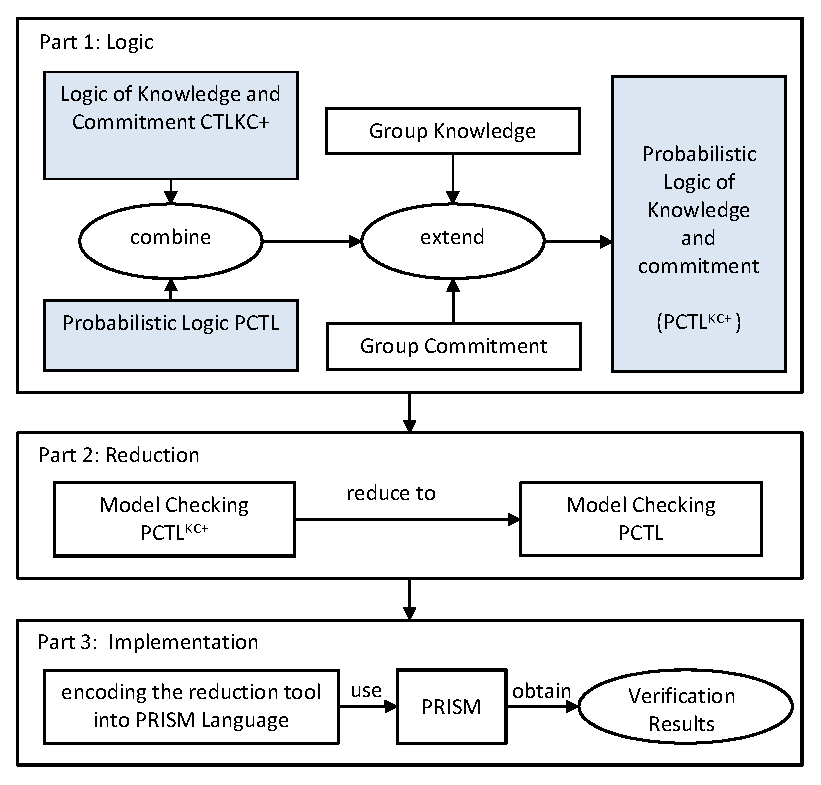
\includegraphics[width=14cm, height=10cm]{chap5/img/approach-cha5-new.eps}
                \end{center}
                \caption{A schematic view of the probabilistic group social commitment approach} \label{fig:approach-PCTLKC+}
                \label{Stack}
                \end{figure}



\section{The New Probabilistic Logic of knowledge and Commitment (PCTL$^{\textrm{kc+}}$)} \label{sec:logic}

To overcome the inconsistency problem of PCTL$^{kc}$, we develop a new logic called the new probabilistic logic of knowledge and commitment (PCTL$^{\textrm{kc+}}$). To build PCTL$^{\textrm{kc+}}$, there are two obvious resources available in the literature: 1) the traditional temporal logics that have been developed for knowledge and social commitments independently or together such as CTLC \cite{Bentahar2012}, CTLK \cite{Lomuscio2007}, and CLTKC$^+$ \cite{Al-Saqqar2014a}; and 2) the existing probabilistic logics available in the literature such as PCTL \cite{Hansson1994}, PCLTK \cite{Wan2013}, and PCTLC \cite{Sultan2014a}. Unfortunately, none of these resources is perfectly suitable for the task. The former resource neglects the uncertainty aspects in MASs, while the
latter doesn't capture the interaction between knowledge and
social commitments. Therefore, we propose a solution that draws
upon both resources. In particular, we combine an existing
consistent logic of knowledge and commitment CTLKC$^+$
\cite{Al-Saqqar2014a} with a well established probabilistic
temporal logic PCTL \cite{Hansson1994}. Then, we extend the
resulting combined logic by adding new operators for the group knowledge
and group commitment.

Before going further, let us first describe a new probabilistic model over which PCTL$^{\textrm{kc+}}$ formulae can be interpreted. This model is an extension of the formalism of interpreted systems
\cite{Fagin1995} with the concepts of epistemic accessibility and
social accessibility relations. Concretely, the model of PCTL$^{\textrm{kc+}}$ is generated from combining two extended versions of the interpreted systems formalism. These extended formalisms are the extended version introduced in \cite{Halpern2003,Wan2013} and a modified version of the extended version given in \cite{Bentahar2012,El-Menshawy2013a} due to Al-Saqqar et al. \cite{Al-Saqqar2014a}.


\begin{definition} [PCTL$^{\textrm{kc+}}$ Model] ~\label{dfn:Models}

\noindent Given a set of atomic propositions $\Phi_p = (p,q,r, \ldots)$ and a set of agents $\texttt{Agt}=\{1,\ldots,n\}$,  the model $\mathfrak{M_3}=(S,\textbf{P},I,\sim_1, \ldots
,\sim_n,\{\approx_{i \rightarrow j}\}_{{(i,j)}\in \texttt{Agt}^2},\nu)$ is a tuple where:
%
\begin{itemize}
\item  $S \subseteq L_1 \times \ldots \times L_n$ is a countable set of all reachable global states of the system. A state $s$ is reachable iff there exists a sequence of transitions from an initial state to $s$ in which the probability of each transition is greater than $0$.

\item  $I \in S$ is an initial global state for the system.


\item  $\textbf{P}:S\times S\rightarrow [0,1]$ is a total transition probability function defined as $\textbf{P}(s, s')=\tau(s,a^{s \rightarrow s'}, s')$ iff there exists a joint action $a=(a_1,\ldots,a_n) \in ACT$ such that\\
     $\sum_{i \in \texttt{Agt}} \tau_i(l_i(s),a^{l_i(s)\rightarrow l_i(s')},l_i(s')) > 0$ and $\sum_{s' \in S} \textbf{P}(s,s') =1$ for all $s \in S$.

\item  $\sim_i \subseteq S \times S$ is the epistemic accessibility relation for the agent $i$, such that for two global states $s$ and $s'$, we have: $s \sim_i s'$ iff $l_i(s)=l_i(s')$.

\item For each pair $(i,j) \in \texttt{Agt}^2$, $\approx_{i\rightarrow j} \subseteq S \times S$ is the social accessibility relation which is defined as follows: $ s \approx_{i\rightarrow j} s' $ iff $ Var_i \cap Var_j \neq \emptyset $ such that $ \forall x \in Var_i \cap Var_j $ we have $ l_i^x(s) = l_i^x(s') = l_j^x(s')$.

\item  $\nu : S \rightarrow 2 ^{\Phi_p} $ is a valuation function.

\end{itemize}
\end{definition}
%

The new model $\mathfrak{M_3}$ differs from the model $\mathfrak{M_2}$,  presented in Chapter \ref{cha:PCTLKC}, in one particular point which is the social accessability relation. While $\mathfrak{M_2}$ uses the social accessibility relation $\sim_{i\rightarrow j}$ that has been introduced in \cite{Bentahar2012,El-Menshawy2013a}, the new model adopts the one $\approx_{i\rightarrow j}$ proposed in \cite{Al-Saqqar2014a} in order to overcome the over-specification problem appeared in $\sim_{i\rightarrow j}$.



\subsection{Syntax of PCTL$^{\textrm{kc+}}$} \label{def:syntax-PCTLKC+}

\begin{definition}[PCTL$^{\textrm{kc+}}$ syntax]\label{def:syntax-PCTLKC+}
Let $\Phi_p=\{p,q, \dots\}$ be a set of atomic propositions, and $\texttt{Agt}=\{1, \dots, n\}$ be a set of agents. The syntax of PCTL$^{\textrm{kc+}}$, which is a combination of PCTLK \cite{Wan2013} and PCTLC \cite{Sultan2014a,Sultan2013} augmented with further operators for the group knowledge, is given by the following grammar:

\vspace{-0.5cm}
\begin{align*}
    \varphi & ::= p~|~\neg \varphi~|~\varphi \vee \varphi~|~\mathcal{K}~|~\mathcal{C}~|~ \mathbb{P}_{\bowtie k} (\psi)~|~\mathbb{P}_{\bowtie k}(\mathcal{K})|~\mathbb{P}_{\bowtie k}(\mathcal{C})\\
    \psi & ::=\bigcirc \varphi ~ | ~ \varphi ~U~ \varphi~|~ \varphi~ U^{\leq m} ~ \varphi \\
    \mathcal{K} & ::= K_i ~\varphi ~|~ E_{G} ~\varphi\\
    \mathcal{C} & ::= C_{i\rightarrow j} ~\varphi ~| ~ C_{i\rightarrow G} ~\varphi ~| ~Fu(C_{i\rightarrow j} ~\varphi) ~| ~Fu(C_{i\rightarrow G} ~\varphi)
\end{align*}
%
where;\\
\noindent -- $p\in\Phi_p$ is an atomic proposition\\
\noindent -- $i,j \in \texttt{Agt}$.\\
\noindent -- $G\subseteq \texttt{Agt}$.\\
\noindent -- $\mathbb{P}_{\bowtie k}$ is a probabilistic operator and $\bowtie \in\{<,\leq,>,\ge\}$.\\
\noindent -- $k\in [0,1]$ is a probability bound or threshold.\\
$m \in\mathbb{N}^+ $ is a positive integer number reflecting the maximum number of transitions needed to reach a certain state.\\
\noindent -- The Boolean connectives $\neg$ and $\vee$ are defined in the usual way.\\
\noindent -- $\varphi$ and $\psi$ are state and path formulae interpreted over the states and paths of $\mathfrak{M_3}$ respectively.\\
\noindent -- The modal connectives $\mathcal{K}$ and $\mathcal{C}$ stand for ``epistemic" and ``social" operators, respectively.\\

\end{definition}
\vspace{-0.5cm}

\noindent In this logic, formulae $\mathcal{K}$ are state formulae and used to express the epistemic properties through the operators; $K_i$ which stands for agent $i$ knows, $E_G$ which stands for everyone knows. Modal connectives $C_{i\rightarrow j}$ and $C_{i\rightarrow G}$ are called social formulae and stand for ``commitment'' from a debtor towards a single creditor, and ``commitment'' from a debtor to a group of creditors, respectively. Likewise, modal connectives $Fu(C_{i\rightarrow j})$ and $Fu(C_{i\rightarrow G})$ stand for ``fulfillment'' of the commitment $C_{i\rightarrow j}$ and ``fulfillment'' of the commitment $C_{i\rightarrow G}$, respectively. $\bigcirc, U$ and $U^{\leq m}$ stand for ``next time'', ``until'' and ``bounded until'' path modal connectives respectively.

%%%%%%%%%%%%%%%%%%%%%%%%%%%%%%%%%%%%%%%%%%%%%%%%%%%%%%%%%%%%%%%%%%%%%%%%%%%%%
%%%%%%%%%%%%%%%%%%%%%%%%%%%%%%%%%%%%%%%%%%%%%%%%%%%%%%%%%%%%%%%%%%%%%%%%%%%%%


\subsection{Social Commitments Classification} \label{sec:commitment-classification}



Social commitments for agent communication have been always looked
at within the scope of one-to-one. However,
back to our motivating example, we realize that in addition to the
usual agent-to-agent scheme, there are certain situations where
group-agent commitments are needed. In this chapter, we are
interested to move beyond the scope of one-to-one and
investigate the case of committing to multiple agents. The idea of
investigating other schemes of social commitments rather than the
one-to-one commitment scheme seems to be both technically
interesting and intuitively appealing. In what follows, we
distinguish between two different flavors of social commitments,
namely basic (or individual) social commitment and group social
commitment.

\begin{definition} [Basic Social Commitment]~

A basic social commitment is an agreement between two agents
namely, \texttt{debtor} and \texttt{creditor} such that the
\texttt{debtor} engages towards the \texttt{creditor} to bring
about a certain property.
\end{definition}

This is the simplest form of social commitments and has long been
investigated in the literature. The commitment in this case can be
represented using the following operator: $C_{i\to j} ~\varphi$
where $i$ denotes the debtor, $j$ denotes the creditor, and
$\varphi$ denotes the content of the commitment. The fulfillment
of such a commitment is written as follows: $Fu(C_{i\to j}
~\varphi)$. However, as the common form of social commitments is
the basic social commitment, we can simply use ``social
commitments" to refer to ``basic (or individual) social
commitments".


\begin{definition} [Group Social Commitment]~

A group social commitment is an agreement between a
\texttt{debtor} and a group of \texttt{creditors} to bring about a
certain property.
\end{definition}

This kind of commitments indicates the involvement of multiple
agents in the same commitment. The creditor is a group of
independent agents that join together as a single party due to
their shared interests in the commitment at hand. A group social
commitment is represented using the following notation: $C_{i\to
G} ~\varphi$, where $i$ denotes the debtor, $G$ denotes a group of
creditors, and $\varphi$ denotes the content of the commitment.
The fulfillment of such a commitment is given by the notation
$Fu(C_{i\to G} ~\varphi)$. Technically, a group social commitment
can be seen as the conjunction of individual basic social
commitments from the debtor $i$ to each agent in the group of
creditors $G$. Formally, $C_{i\to G} ~\varphi \equiv
\bigwedge\limits_{j\in G} C_{i\rightarrow j} ~\varphi$. An
intuitive explanation of the operator $C_{i\to G} ~\varphi$ is as
follows: for a group social commitment to be held at a certain
state, the content of the commitment must be true at every
accessible state from the commitment state with respect to the
group. This implies that none of the group members could be
excluded from having all accessible states satisfy the content of
the commitment. Consequently, it is obvious that for a state to be
socially accessible from the commitment state with respect to the
group, it has to be socially accessible with respect to at least
one of the agents of the group. Therefore, we resolve the
accessibility problem resulted from having group commitments by
taking the union of the social accessibility relations of each
single agent in the group. This in turn leads us to define the
group social accessibility relation based on the social
accessibility relations presented in Definition \ref{dfn:Models}.


Let $G\subseteq \texttt{Agt}$ be a group of agents. We define the group social accessibility relation from the social accessibility relation $\approx_{i \to j}$ as follows:
\begin{definition} [Social Accessibility Relations for Group Social Commitment] \label{dfn: group social
relations}~
%
\begin{itemize}

\item $\approx_{i \rightarrow G}$ is the union of the social accessibility relations between agent $i$ and each agent in the group $G$: $\approx_{i \to G}=\bigcup\limits_{j \in G}\approx_{i\to j}$.

\end{itemize}

\end{definition}


\begin{figure}[t]
                \begin{center}
                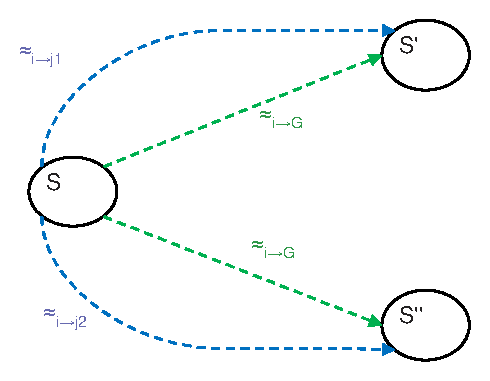
\includegraphics[width=7cm, height=5cm]{chap5/img/group-sc.eps}
                \end{center}
                \caption{Accessibility relations for group social commitment} \label{fig:group-sc}
                \end{figure}

Notice that group social commitments have all the properties of basic social commitments with an additional constraint that they can involve more than two agents. However, a group social commitment involving only two agents is equivalent to the basic social commitment. Figure \ref{fig:group-sc} depicts the idea of group social accessibility ($G=\{j_1, j_2\}$).

\subsection{Group Knowledge}  \label{sec:Group Knowledge}
In this work, we limit the scope of group knowledge to the concept of ``Everyone Knows" introduced in \cite{Fagin1995}. ``Everyone Knows" is denoted by $E_G ~\varphi$ and means that everyone in the group $G$ knows $\varphi$. Technically, ``Everyone knows" can be seen as the conjunction of the individual knowledge of each agent in the group. Formally, $E_G ~\varphi \equiv \bigwedge\limits_{i\in G} K_i ~\varphi$.

Before we proceed to present the semantics of
PCTL$^{\textrm{kc+}}$, we need to define the epistemic
accessibility relation for $E_G ~\varphi$. Let $G\subseteq
\texttt{Agt}$ be a group of agents. We define the epistemic
accessibility relation for $E_G ~\varphi$ from the epistemic
accessibility relation $\sim_i$ as follows \cite{Wan2013}:\\

\begin{definition} [Epistemic Accessibility Relation for Everyone Knows] \label{dfn: epistemic relations}~
\begin{itemize}

\item $\sim_G^{E}$ is the union of group $G's$ accessibility
relations: $\sim_G^{E}=\bigcup\limits_{i \in G}\sim_i$.

\end{itemize}
\end{definition}

\subsection{Semantics of PCTL$^{\textrm{kc+}}$} \label{def:semantics-PCTLKC+}

Given a model $\mathfrak{M_3}=(S,\textbf{P},I,\sim_1, \ldots
,\sim_n,\{\approx_{i \to j}\}_{{(i,j)}\in \texttt{Agt}^2},\nu)$, then $(\mathfrak{M_3},s) \models \varphi$ states that ``a state $s$ in the model $\mathfrak{M_3}$ satisfies a state formula $\varphi$, $(\mathfrak{M_3},\pi) \models \psi$ means that ``a path $\pi$ in the model $\mathfrak{M_3}$ satisfies a path formula $\psi$, and
$(\mathfrak{M_3},s) \models \mathbb{P}_{\bowtie k}(\psi)$ means that
``a state $s$ in $\mathfrak{M_3}$ satisfies
$\mathbb{P}_{\bowtie k}(\psi)$ if the probability of taking a path
from $s$ that satisfies $\psi$ is in the interval specified by
$\bowtie k$''. When the model $\mathfrak{M_3}$ is clear from the
context, we simply write the satisfaction relation $\models$ as
follows: $s \models \varphi$ and $\pi \models \psi$. Furthermore,
we denote the number of socially accessible states $s'$ from a given state $s$ such that $s\approx_{i\to j}s'$ by $|s\approx_{i\to j}s'|$, and $s\approx_{i\to G}s'$ by $|s\approx_{i\to G}s'|$.
We also denote the number of epistemically accessible states $s'$ from a given state $s$ such that $s\sim_i s'$ by $|s\sim_i s'|$. Similarly, we
denote the number of states $s'$ that are accessible from a given
state $s$ through $\sim_G^E$ by $|s\sim_G^E s'|$.
Finally, we define $|s\models \varphi|$ as follows:

\begin{center}
$|s\models \varphi|=
\begin{cases}
1,~~~\textrm{if}~ s\models\varphi\\
0,~~~\textrm{otherwise}.
\end{cases}$
\end{center}


%
\begin{definition}[\textbf{Satisfaction}]\label{def:semantics-pctlkc+} Satisfaction of a PCTL$^{\textrm{kc+}}$ formula in the model $\mathfrak{M_3}$ is conductively defined as follows:



\noindent $s\models p~~~~~~~~~~~~~~~~~~~\emph{iff}~~p\in \nu(s);\\
s\models \varphi_1 \vee \varphi_2 ~~~~~~~~\emph{iff}~~s\models \varphi_1~\textrm{or}~s \models \varphi_2; \\
s\models \neg \varphi~~~~~~~~~~~~~~~~\emph{iff}~~s \nvDash \varphi;\\
s\models K_i \varphi  ~~~~~~~~~~~~~~ \emph{iff}~~ \forall s'\in S ~ \textrm{s.t.} ~~ s \sim_i s',  \ \textrm{we~have}~ s'\models \varphi; \\
s\models E_G ~\varphi ~~~~~~~~~~~~ \emph{iff}~~\forall s'\in S~ \textrm{s.t.} ~~ s\sim_G^E s', \ \textrm{we~have}~ s'\models \varphi; \\
s\models C_{i\rightarrow j} \varphi  ~~~~~~~~~~ \emph{iff} ~~\forall s' \in S~\textrm{s.t.}~~s \approx_{i \rightarrow j}s', \textrm{we~have}~s'\models K_i \varphi \wedge K_j \varphi;\\
s\models C_{i\rightarrow G} \varphi  ~~~~~~~~~ \emph{iff} ~~\forall s' \in S~\textrm{s.t.}~~s \approx_{i \rightarrow G}s', \textrm{we~have}~s'\models K_i \varphi \wedge E_G ~\varphi $;\\
$s\models Fu(C_{i\rightarrow j} \varphi)$ ~\emph{iff} there exists $ s' \in S $ such that $ s' \approx_{i \rightarrow j} s $ and $~s'\models C_{i\rightarrow j} ~\varphi$ or \\
$~~~~~~~~~~~~~~~~~~~~~~~~~~~~~~~~~~~$there exists $ s'' \in S $ and $ s'' \sim_i s $ such that $~s''\models Fu(C_{i\rightarrow j} ~\varphi)$ or \\
$~~~~~~~~~~~~~~~~~~~~~~~~~~~~~~~~~~~$there exists $ s'' \in S $  and $ s'' \sim_j s $ such that $~s''\models Fu(C_{i\rightarrow j} ~\varphi)$;\\
$s\models Fu(C_{i\rightarrow G} ~\varphi)$ ~\emph{iff} there exists $ s' \in S $ such that $ s' \approx_{i \rightarrow G} s $ and $~s'\models C_{i\rightarrow G} ~\varphi$ or \\
$~~~~~~~~~~~~~~~~~~~~~~~~~~~~~~~~~~~$there exists $ s'' \in S $ and $ s'' \sim_i s $ such that $~s''\models Fu(C_{i\rightarrow G} ~\varphi)$ or \\
$~~~~~~~~~~~~~~~~~~~~~~~~~~~~~~~~~~~$there exists $ s'' \in S $  and $ s'' \sim_G^E s $ such that $~s''\models Fu(C_{i\rightarrow G} ~\varphi)$;\\
\noindent $\pi \models \bigcirc \varphi~~~~~~~~~~~~~~\emph{iff}~~\pi(1) \models \varphi; \\
\pi \models \varphi_1~U^{\leq m}~\varphi_2~~\emph{iff}~~\exists k \leq m~~\textrm{s.t.}~~ \pi(k) \models \varphi_2 ~\textrm{and}~\forall i < k, \pi(i) \models \varphi_1;\\
\pi \models \varphi_1 ~U~\varphi_2~~~~~~~\emph{iff}~~\exists m \geq 0~~\textrm{s.t.}~~\pi \models \varphi_1~U^{\leq m}~\varphi_2;$\\
\noindent $s \models \mathbb{P}_{\bowtie k} (\psi)~~~~~~~~~\emph{iff}~~Prob_s(\psi)\bowtie k$ where: $Prob_s(\psi)=Prob_s\{\pi \in \Pi(s)~|~\pi\models
\psi\};$\\


\noindent $\bullet$ For a probabilistic operator working on an epistemic formula, where the set of all accessible states from $s$ is our sample space and the set of events $\mathrm{F}$ is the set of states accessible from $s$ and satisfy the formula:


\begin{tabbing}
\noindent $s\models \mathbb{P}_{\bowtie k}(K_i~\varphi) $
    \ \ \ \ \ \= \emph{iff} \ $Prob(s \models K_i\varphi)$ $\bowtie k$ where: $Prob(s\models K_i\varphi)=\frac{\sum_{s \sim_i s'}|s'\models \varphi| }{|s \sim_i s'|};$
\end{tabbing}

\begin{tabbing}
 \noindent $s\models \mathbb{P}_{\bowtie k}(E_G~\varphi) $
    \ \ \ \ \ \= \emph{iff} \ $Prob(s \models E_G~\varphi)$ $\bowtie k$ where: $Prob(s\models E_G~\varphi)=\frac{\sum_{s \sim_G^E s'}|s'\models \varphi| }{|s \sim_G^E s'|};$

\end{tabbing}


\noindent $\bullet$  For a probabilistic operator working over a commitment formula,where the set of all accessible states from $s$ is our sample space and the set of events $\mathrm{F}$ is the set of states accessible from $s$
and satisfy the formula: \\


\noindent $s\models \mathbb{P}_{\bowtie k}(C_{i\rightarrow j}\varphi)$
   ~~\emph{iff}  $Prob(s \models C_{i\rightarrow j}\varphi) \bowtie \!k$ where: $Prob(s\models C_{i\rightarrow j}\varphi)=\frac{\sum_{s \approx_{i \rightarrow j}s'}|s'\models K_i \varphi \wedge K_j \varphi| }{|s \approx_{i \rightarrow j}s'| };$\\

\noindent $s\models \mathbb{P}_{\bowtie k}(C_{i\rightarrow G}\varphi)$
   ~\emph{iff}  $Prob(s \models C_{i\rightarrow G}\varphi) \bowtie \!k$ where: $Prob(s\models C_{i\rightarrow G}\varphi)=\frac{\sum_{s \approx_{i \rightarrow G}s'}|s'\models K_i \varphi \wedge E_G \varphi| }{|s \approx_{i \rightarrow G}s'| };$\\


\noindent $\bullet$ For a probabilistic operator working over a fulfilment formula, assuming that accessible states are also reachable:\\


\noindent $s\models \mathbb{P}_{\bowtie k}(Fu(C_{i\rightarrow j}\varphi))$
    ~~ \emph{iff}~ $Prob(s \models Fu(C_{i\rightarrow j}\varphi)) \bowtie k;$ where:

\vspace{-0.4cm}
\begin{align*}
%%
& Prob(s\models Fu(C_{i\rightarrow j}\varphi))\ = Prob_s\{\pi \in \Pi(s') ~|~s' \approx_{i \rightarrow j}s ~\textrm{and}~ \pi = s' \ldots s ~\textrm{and}~ s' \models C_{i\rightarrow j}\varphi\};
\end{align*}

\noindent $s\models \mathbb{P}_{\bowtie k}(Fu(C_{i\rightarrow G}\varphi))$
    ~~ \emph{iff}~ $Prob(s \models Fu(C_{i\rightarrow G}\varphi)) \bowtie k;$ where:

\vspace{-0.4cm}
\begin{align*}
%%
& Prob(s\models Fu(C_{i\rightarrow G}\varphi))\ = Prob_s\{\pi \in \Pi(s') ~|~
& s' \approx_{i \rightarrow G}s ~\textrm{and}~ \pi = s' \ldots s ~\textrm{and}~ s' \models C_{i\rightarrow G}\varphi\}
\end{align*}

\end{definition}

Again as in Chapter \ref{cha:PCTLKC}, in the case of the knowledge, the uncertainty is computed in such a way that it reflects the indistinguishability property of the epistemic accessibility relations. Hence, the uncertainty is computed based on the probability of epistemic accessibility relations which is calculated based on the number of accessible states satisfying the content of the knowledge over the number of equivalent states, as all the states are equally accessible. Likewise, probabilistic commitment is computed based on the number of accessible states that satisfy the content over the whole number of accessible states, which demonstrates the uncertainty of the agent over the accessible states, so that over the commitment. Probabilistic fulfillment, however, is computed using the probabilistic transitions of the path linking the commitment state to the fulfillment state.

The following proposition is straightforward from the semantics:

\begin{proposition} \label{proposition}~\\
If $(\mathfrak{M_3},s)\models \mathbb{P}_{\leq0} (Fu(C_{i \rightarrow
j}\varphi))$ and $(\mathfrak{M_3},s)\models Fu(C_{i \rightarrow
j}\varphi)$, then $s$ is not reachable from the commitment state.
\end{proposition}


\begin{theorem} [Epistemic Equivalences]\label{theorm:Epistemic-equivalence} \ \ \ \

    \begin{enumerate}
        \item $(\mathfrak{M_3},s)\models \mathbb{P}_{\geq1}(K_i~\varphi)$  ~~~~~~iff~~  $(\mathfrak{M_3},s) \models K_i~\varphi$
        \item $(\mathfrak{M_3},s)\models \mathbb{P}_{\leq 0}(K_i~\varphi)$   ~~~~~~iff~~  $(\mathfrak{M_3},s)\models K_i ~\neg \varphi$
        \item $(\mathfrak{M_3},s)\models \mathbb{P}_{]0,1[}(K_i~\varphi)$  ~~~~iff~~   $(\mathfrak{M_3},s)\models \neg K_i~\neg\varphi \wedge \neg K_i~\phi$
        \item $(\mathfrak{M_3},s)\models \mathbb{P}_{\geq1}(E_G~\varphi)$  ~~~~iff~~  $(\mathfrak{M_3},s) \models E_G~\varphi$
        \item $(\mathfrak{M_3},s)\models \mathbb{P}_{\leq 0}(E_G~\varphi)$   ~~~~iff~~  $(\mathfrak{M_3},s)\models E_G ~\neg \varphi$
        \item $(\mathfrak{M_3},s)\models \mathbb{P}_{]0,1[}(E_G~\varphi)$  ~~iff~~   $(\mathfrak{M_3},s)\models \neg E_G~\neg\varphi \wedge \neg E_G~\varphi$

    \end{enumerate}

\end{theorem}


\begin{proof} %\hspace{-0.9cm}
We prove the first three equivalences, the same method can be used to prove the others.
\begin{itemize}
\item First equivalence. ~\\
    $``\Rightarrow"$. Assume $(\mathfrak{M_3},s)\models \mathbb{P}_{\geq1} (K_i\varphi)$.
    By the semantics of PCTL$^{\textrm{kc+}}$, it follows that $Prob((\mathfrak{M_3},s)\models K_i~\varphi)\geq1$.
    Therefore, $\frac{\sum_{s\sim_i s'}|(\mathfrak{M_3},s')\models \varphi| }{|s\sim_i s'|}\geq1$. This means that $\forall s'\in S$ such that $s\sim_i s'$, we have $(\mathfrak{M_3},s')\models \varphi$ (as $\sim_i$ is reflexive, so $s'$ could be $s$ itself). Thus, $(\mathfrak{M_3},s) \models K_i ~\varphi$. \\
    $``\Leftarrow"$. Assume $(\mathfrak{M_3},s)\models K_i~\varphi$. By the PCTL$^{\textrm{kc+}}$ semantics, it follows that for all $s'\in S$ such that $s\sim_i s'$, we have $(\mathfrak{M_3},s')\models \varphi$ (i.e. all accessible states from $s$ satisfy $\varphi$).
    Consequently, $\sum_{s\sim_i s'}|(\mathfrak{M_3},s')\models \varphi| = |s\sim_i s'|$.
    Therefore, $\frac{\sum_{s\sim_i s'}|(\mathfrak{M_3},s')\models \varphi| }{|s\sim_i s'|}\geq1$ and hence $(\mathfrak{M_3},s)\models \mathbb{P}_{\geq1} K_i\varphi)$.

\item Second equivalence. ~\\
    $``\Rightarrow"$. Assume $(\mathfrak{M_3},s)\models \mathbb{P}_{\leq0} (K_i\varphi)$.
    By the PCTL$^{\textrm{kc+}}$ semantics, it follows that $Prob((\mathfrak{M_3},s)\models K_i\varphi)\leq0$.
    Thus, $\frac{\sum_{s\sim_i s'}|(\mathfrak{M_3},s')\models \varphi|}{|s\sim_i s'|}\leq0$. Since $\sim_i$ is reflexive, so the set of the accessible states from $s$ is not empty. Therefore, $\sum_{s\sim_i s'}|(\mathfrak{M_3},s')\models \varphi|$ must be 0 (i.e., $\varphi$ is not true in any of the accessible states). Consequently, for all $s'\in S$ such that $s\sim_i s'$, we have $(\mathfrak{M_3},s')\nvDash \varphi$, which means $(\mathfrak{M_3},s')\models \neg \varphi$. Hence, $(\mathfrak{M_3},s)\models K_i \neg \varphi$.~\\
%
    $``\Leftarrow"$. Assume $(\mathfrak{M_3},s)\models K_i\neg \varphi$. By the PCTL$^{\textrm{kc+}}$ semantics, it follows that $\forall s'\in S$ such that $s\sim_i s'$, we have $(\mathfrak{M_3},s')\nvDash \varphi$. Since the set of the accessible states from $s$ is not empty, then $\frac{\sum_{s\sim_i s'}|(\mathfrak{M_3},s')\models \varphi| }{|s\sim_i s'|}\leq0$. Hence, $(\mathfrak{M_3},s)\models \mathbb{P}_{\leq0} (K_i\varphi)$.

\item Third equivalence. ~\\
    $``\Rightarrow"$. Assume $(\mathfrak{M_3},s)\models \mathbb{P}_{]0,1[} K_i\varphi)$. By the PCTL$^{\textrm{kc+}}$ semantics, it follows that $0< Prob(s\models K_i\varphi)<1$. Thus, $0<\frac{\sum_{s\sim_i s'}|(\mathfrak{M_3},s')\models \varphi| }{|s \sim_i s'|}<1$.
    This means that it would never be the case that $\sum_{s\sim_i s'}|(\mathfrak{M_3},s')\models \varphi| = |s\sim_i s'|$ nor $\sum_{s\sim_i s'}|(\mathfrak{M_3},s')\models \varphi| = 0$. Consequently, there exist some $s', s'' \in S$ such that $s\sim_i s'$ and $s\sim_i s''$ and $(\mathfrak{M_3},s')\models \varphi$ and $(\mathfrak{M_3},s'')\models \neg \varphi$. Hence, it is impossible to have $(\mathfrak{M_3},\overline{s})\models \neg\varphi$ or $(\mathfrak{M_3},\overline{s})\models \varphi$ for all $\overline{s}\in S$ such that $s\sim_i \overline{s}$. Consequently, $(\mathfrak{M_3},s)\nvDash K_i\neg\varphi$ and $(\mathfrak{M_3},s)\nvDash K_i\varphi$. Hence $(\mathfrak{M_3},s)\models \neg K_i\neg\varphi$ and $(\mathfrak{M_3},s)\models \neg K_i\varphi$. ~\\
    %
    $``\Leftarrow"$. Assume $(\mathfrak{M_3},s)\models \neg K_i\varphi$. By the PCTL$^{\textrm{kc+}}$ semantics, it follows that there exists $s'\in S$ such that $s\sim_i s'$ and $(\mathfrak{M_3},s')\models \neg \varphi$. Consequently, it would never be the case that for all $s'\in S$ such that $s\sim_i s'$ we have $(\mathfrak{M_3},s')\models \varphi$. Therefore, $1>\frac{\sum_{s\sim_i s'}|(\mathfrak{M_3},s')\models \varphi| }{|s\sim_i s'|}$. Now assume $(\mathfrak{M_3},s)\models \neg K_i\neg \varphi$. Therefore, $\sum_{s\sim_i s'}|(\mathfrak{M_3},s')\models \varphi| = 0$ would never be the case as some accessible states should satisfy $\varphi$. Consequently, $\frac{\sum_{s\sim_i s'}|(\mathfrak{M_3},s')\models \varphi| }{|s\sim_i s'|}>0$. Thus, $0<\frac{\sum_{s\sim_i s'}|(\mathfrak{M_3},s')\models \varphi| }{|s \sim_i s'|}<1$. Hence, $(\mathfrak{M_3},s)\models \mathbb{P}_{]0,1[} (K_i\varphi)$.
\end{itemize}
\end{proof}


%%%%%%%%%%%%%%%%%%%%%%%%%%%%%%%%%%%%%%%%%%%%%%%%%%%%%%%%%%%%%%%%%%

\begin{theorem} [Commitment Equivalences] \label{theorem:Commitment-Equivelances} ~

\begin{enumerate}
\item $(\mathfrak{M_3},s)\models \mathbb{P}_{\geq1} (C_{i \rightarrow
j}\varphi)$ ~~~~~iff~~ $(\mathfrak{M_3},s)\models C_{i \rightarrow
j}\varphi$

\item $(\mathfrak{M_3},s)\models \mathbb{P}_{\leq0} (C_{i \rightarrow
j}\varphi)$ ~~~~~iff~~ $(\mathfrak{M_3},s)\models C_{i \rightarrow
j}\neg \varphi$

\item $(\mathfrak{M_3},s)\models \mathbb{P}_{]0,1[} (C_{i \rightarrow
j}\varphi)$ ~~~iff~~ $(\mathfrak{M_3},s)\models \neg C_{i
\rightarrow j}\neg\varphi \wedge \neg C_{i \rightarrow j}\varphi$

\item $(\mathfrak{M_3},s)\models \mathbb{P}_{\geq1} (C_{i \rightarrow
G}\varphi)$ ~~~~iff~~ $(\mathfrak{M_3},s)\models C_{i \rightarrow
G}\varphi$

\item $(\mathfrak{M_3},s)\models \mathbb{P}_{\leq0} (C_{i \rightarrow
G}\varphi)$ ~~~~iff~~ $(\mathfrak{M_3},s)\models C_{i \rightarrow
G}\neg \varphi$

\item $(\mathfrak{M_3},s)\models \mathbb{P}_{]0,1[} (C_{i \rightarrow
G}\varphi)$ ~~iff~~ $(\mathfrak{M_3},s)\models \neg C_{i
\rightarrow G}\neg\varphi \wedge \neg C_{i \rightarrow G}\varphi$

\end{enumerate}

\end{theorem}

\begin{proof}
We prove the first three equivalences, the same method can be used to prove the others.

\begin{itemize}
\item First equivalence. ~\\
    $``\Rightarrow"$. Assume $(\mathfrak{M_3},s)\models \mathbb{P}_{\geq1} (C_{i \rightarrow j}\varphi)$.
    By the PCTL$^{\textrm{kc+}}$ semantics, it follows that $Prob((\mathfrak{M_3},s)\models C_{i\rightarrow j}\varphi)\geq1$.
    Thus,  $\frac{\sum_{s\approx_{i \rightarrow j}s'}|(\mathfrak{M_3},s')\models \varphi| }{|s\approx_{i \rightarrow j}s'|}\geq1$.
    This means that for all $s'\in S$ such that $s\approx_{i \rightarrow j}s'$, we have $(\mathfrak{M_3},s')\models \varphi$, and hence $(\mathfrak{M_3},s) \models C_{i\rightarrow j}\varphi$. \\
    $``\Leftarrow"$. Assume $(\mathfrak{M_3},s)\models C_{i \rightarrow j}\varphi$. By the PCTL$^{\textrm{kc+}}$ semantics, it follows that for all $s'\in S$ such that $s\approx_{i \rightarrow j}s'$,
    we have $(\mathfrak{M_3},s')\models \varphi$ (i.e. all accessible states from $s$ satisfy $\varphi$).
    Consequently, $\sum_{s\approx_{i \rightarrow j}s'}|(\mathfrak{M_3},s')\models \varphi| = |s\approx_{i \rightarrow j}s'|$.
    Therefore, $\frac{\sum_{s\approx_{i \rightarrow j}s'}|(\mathfrak{M_3},s')\models \varphi| }{|s\approx_{i \rightarrow j}s'|}\geq1$
    and hence, $(\mathfrak{M_3},s)\models \mathbb{P}_{\geq1} (C_{i \rightarrow j}\varphi)$.

\item Second equivalence. ~\\
    $``\Rightarrow"$. Assume $(\mathfrak{M_3},s)\models \mathbb{P}_{\leq0} (C_{i \rightarrow j}\varphi)$.
    By the PCTL$^{\textrm{kc+}}$ semantics, it follows that $Prob((\mathfrak{M_3},s)\models C_{i\rightarrow j}\varphi)\leq0$.
    Thus, $\frac{\sum_{s\approx_{i \rightarrow j}s'}|(\mathfrak{M_3},s')\models \varphi|}{|s\approx_{i \rightarrow j}s'|}\leq0$.
    Since the set of the accessible states from $s$ is not empty, then $\sum_{s\approx_{i \rightarrow j}s'}|(\mathfrak{M_3},s')\models \varphi|$
    must be 0 (i.e. $\varphi$ is not true in any of the accessible states). Consequently, for all $s'\in S$ such that $s\approx_{i \rightarrow j}s'$, we have $(\mathfrak{M_3},s')\nvDash \varphi$, which means $(\mathfrak{M_3},s')\vdash \neg \varphi$.
     Hence, $(\mathfrak{M_3},s)\models C_{i\rightarrow j}\neg \varphi$.~\\
%
    $``\Leftarrow"$. Assume $(\mathfrak{M_3},s)\models C_{i \rightarrow j}\neg \varphi$. By the PCTL$^{\textrm{kc+}}$ semantics,
    it follows that for all $s'\in S$ such that
    $s\approx_{i \rightarrow j}s'$, we have $(\mathfrak{M_3},s')\nvDash \varphi$. Since the set of the accessible states from $s$ is not empty, then $\frac{\sum_{s\approx_{i \rightarrow j}s'}|(\mathfrak{M_3},s')\models \varphi| }{|s\approx_{i \rightarrow j}s'|}\leq0$. Hence, $(\mathfrak{M_3},s')\models \mathbb{P}_{\leq0} (C_{i \rightarrow j}\varphi)$.

\item Third equivalence. ~\\
    $``\Rightarrow"$. Assume $(\mathfrak{M_3},s)\models \mathbb{P}_{]0,1[} (C_{i \rightarrow j}\varphi)$. By the PCTL$^{\textrm{kc+}}$ semantics, it follows that $0< Prob((\mathfrak{M_3},s)\models C_{i\rightarrow j}\varphi)<1$. Thus, $0<\frac{\sum_{s\approx_{i \rightarrow j}s'}|(\mathfrak{M_3},s')\models \varphi| }{|s \approx_{i \rightarrow j}s'|}<1$.
    This means that it would never be the case that $\sum_{s\approx_{i \rightarrow j}s'}|(\mathfrak{M_3},s')\models \varphi| = |s\approx_{i \rightarrow j}s'|$
    nor $\sum_{s\approx_{i \rightarrow j}s'}|(\mathfrak{M_3},s')\models \varphi| = 0$. Consequently, there exist some $s', s'' \in S$
    such that $s\approx_{i \rightarrow j}s'$ and $s\approx_{i \rightarrow j}s''$ and $(\mathfrak{M_3},s')\models \varphi$ and $(\mathfrak{M_3},s'')\models \neg \varphi$.
    Hence, it is impossible to have $(\mathfrak{M_3},\overline{s})\models \neg\varphi$ or $(\mathfrak{M_3},\overline{s})\models \varphi$ for all $\overline{s}\in S$ such that $s\approx_{i \rightarrow j}\overline{s}$. Consequently,
    $s\nvDash  C_{i \rightarrow j}\neg\varphi$ and  $(\mathfrak{M_3},s)\nvDash  C_{i \rightarrow j}\varphi$. Hence $(\mathfrak{M_3},s)\models \neg C_{i \rightarrow j}\neg\varphi$ and $(\mathfrak{M_3},s)\models \neg C_{i \rightarrow j}\varphi$. ~\\
    %
    $``\Leftarrow"$. Assume $(\mathfrak{M_3},s)\models \neg C_{i \rightarrow j}\varphi$. By the PCTL$^{\textrm{kc+}}$ semantics, it follows that there exists $s'\in S$ such that $s\approx_{i \rightarrow j}s'$ and $(\mathfrak{M_3},s')\models \neg \varphi$. Consequently, it would never be the case that $(\mathfrak{M_3},s')\models \varphi$ for all $s'\in S$
    such that $s\approx_{i \rightarrow j}s'$. Therefore,
    $1>\frac{\sum_{s\approx_{i \rightarrow j}s'}|(\mathfrak{M_3},s')\models \varphi| }{|s\approx_{i \rightarrow j}s'|}$.
    Now assume $(\mathfrak{M_3},s)\models \neg C_{i \rightarrow j}\neg \varphi$. Therefore, $\sum_{s\approx_{i \rightarrow j}s'}|(\mathfrak{M_3},s')\models \varphi| = 0$ would never be he case as some accessible states should satisfy $\varphi$. Consequently,
    $\frac{\sum_{s\approx_{i \rightarrow j}s'}|(\mathfrak{M_3},s')\models \varphi| }{|s\approx_{i \rightarrow j}s'|}>0$.
    Thus, $0<\frac{\sum_{s\approx_{i \rightarrow j}s'}|(\mathfrak{M_3},s')\models \varphi| }{|s \approx_{i \rightarrow j}s'|}<1$. Thus, $(\mathfrak{M_3},s)\models \mathbb{P}_{]0,1[} (C_{i \rightarrow j}\varphi)$.
\end{itemize}

\end{proof}


%%%%%%%%%%%%%%%%%%%%%%%%%%

\begin{theorem} [Fulfillment Equivalences] \label{theorem:Fulfiilemt-Equivelances} ~

\begin{enumerate}
\item $(\mathfrak{M_3},s)\models \mathbb{P}_{>0} (Fu(C_{i \rightarrow
j}\varphi))$ iff $(\mathfrak{M_3},s)\models Fu(C_{i \rightarrow
j}\varphi)$ and $s$ is reachable from the commitment state.

\item $(\mathfrak{M_3},s)\models \mathbb{P}_{\leq0} (Fu(C_{i \rightarrow
j}\varphi))$ iff $(\mathfrak{M_3},s)\models \neg Fu(C_{i \rightarrow
j}\varphi)$ or $s$ is not reachable from the commitment state.

\item $(\mathfrak{M_3},s)\models \mathbb{P}_{>0} (Fu(C_{i \rightarrow
G}\varphi))$ iff $(\mathfrak{M_3},s)\models Fu(C_{i \rightarrow
G}\varphi)$ and $s$ is reachable from the commitment state.

\item $(\mathfrak{M_3},s)\models \mathbb{P}_{\leq0} (Fu(C_{i \rightarrow
G}\varphi))$ iff $(\mathfrak{M_3},s)\models \neg Fu(C_{i \rightarrow
G}\varphi)$ or $s$ is not reachable from the commitment state.
\end{enumerate}

\end{theorem}

\begin{proof} %\hspace{0.5cm} \\
The proofs of these equivalences are direct from Proposition
\ref{proposition} and the above semantics.

 \end{proof}

 %%%%%%%%%%%%%%%%%%%%%%%%%%%%%%%%%%%%%%%%%%%%%%%%%%%%%%%%%%%%%%%%%%%%%%%%%%%%%%%%%%%

\section{Model Checking PCTL$^{\textrm{kc+}}$ using Reduction} \label{sec:model-checking-pctlkc+}

In this section, we generalize the model checking technique for
the logic of knowledge and social commitments proposed in
Chapter \ref{cha:PCTLKC} to cover more complex cases, such as group
knowledge and group commitment. As we have seen in the previous
section, the semantics of our new logic PCTL$^{\textrm{kc+}}$ is
defined over an extended version of interpreted systems
$\mathfrak{M_3}$. The idea of our proposed verification technique is
based mainly on reducing the problem of model checking
PCTL$^{\textrm{kc+}}$ to the problem of model checking PCTL. This
however involves two processes. First, we define transformation
rules to transform PCTL$^{\textrm{kc+}}$ model ($\mathfrak{M_3}$) to
an MDP model to be suitable for PRISM, the probabilistic model
checker of PCTL. The solution of an MDP comes in the form of an
``adversary'' \cite{Forejt2011} which is described as a mapping
of states to probability distributions over actions. Second, we
construct a set of rules to reduce PCTL$^{\textrm{kc+}}$ formulae
to PCTL formulae.

In a nutshell, our proposed model checking procedure is as follows. Given $\mathfrak{M_3}=(S,\textbf{P},I,\sim_1, \ldots
,\sim_n,\{\approx_{i \rightarrow j}\}_{{(i,j)}\in \texttt{Agt}^2},\nu)$, and PCTL$^{\textrm{kc+}}$ formula $\varphi$, we have to define an MDP model $\mathfrak{M_3'}$ = $\mathscr{F}(\mathfrak{M_3})$ and PCTL formula $\mathscr{F}(\varphi)$ using the transformation function $\mathscr{F}$ such that $\mathfrak{M_3} \models \varphi$ iff $\mathscr{F}(\mathfrak{M_3})\models \mathscr{F}(\varphi)$.


\begin{figure}[h]
\centering
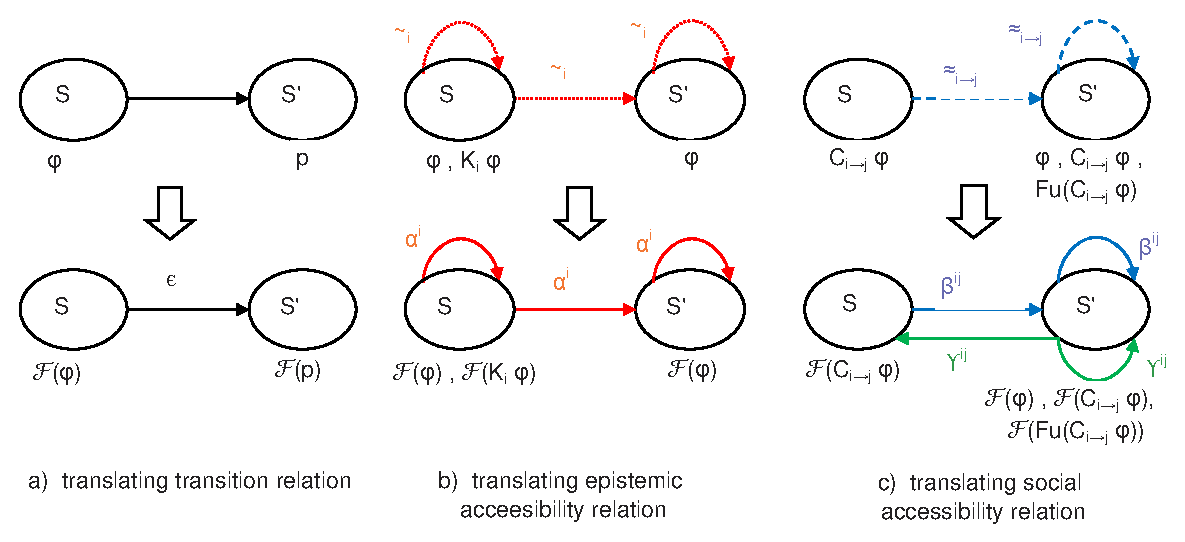
\includegraphics[width=15cm, height=9cm]{chap5/img/relation-translation-cha5.eps}
%height=8cm]{figures/1.eps}
\caption{Examples of translating relations in $\mathfrak{M_3}$ into labeled transitions} \label{fig:relation-translation-cha5}
\end{figure}

%%%%%%%%%%%%%%%%%%%%%%%%%%%%%%%%%%%%%%%%%%%%%%%%%%%%%%%%%%%%%%%%%%%%%%%%%%%%%%

\subsection{Transforming the Model $\mathfrak{M_3}$} \label{sec:reducing-proposed-model-cha5}

As done in Chapter \ref{cha:PCTLKC}, given an MDP model $\mathfrak{M_3'}$ = $(\mathbb{S}, Act, \textsf{P}_t ,I_i, L)$, a major step in transforming $\mathfrak{M_3}$ into $\mathfrak{M_3'}$ is to define the set of actions $Act$. The idea is to map each relation in $\mathfrak{M_3}$ into a corresponding action in $Act$; more specifically, to translate each relation in $\mathfrak{M_3}$ into a labeled transition in $\mathfrak{M_3'}$. Then, these labels (also called actions) are used to form the set $Act$ in $\mathfrak{M_3'}$. Consequently, the different relations in $\mathfrak{M_3}$ namely, probabilistic transition relations, epistemic accessibility relations, and social accessibility relations, are translated into labeled transitions in $\mathfrak{M_3'}$. Moreover, to interpret the fulfillment of a commitment, we need to add the symmetric closure of the transition resulted from translating the social accessibility relation. Figure \ref{fig:relation-translation-cha5} (where $n$ is the number of agents, $1 \leq i \leq n$, and $1 \leq j \leq n$) explains the process of translating the probabilistic transition relation $\textbf{P}$, epistemic accessibility relations $\sim_i$, and social accessibility relations $\approx_{i \to j}$ into labeled transitions. More precisely, the action $\epsilon$ denotes a transition defined from the probabilistic transition relation $\textbf{P}$, action $\alpha^i$ denotes a transition defined from the epistemic accessibility relation $\sim_i$, action $\beta^{ij}$ denotes a transition defined from the social accessibility relation $\approx_{i \rightarrow j}$, and action $\gamma^{ij}$ denotes a transition added to capture the semantics of the fulfillment of a basic commitment. Likewise, the epistemic accessibility relation $\sim_G^E$, and the social accessibility relation $\approx_{i \rightarrow G}$ are translated in the same way where the action $\alpha_G^E$ denotes a transition defined from the epistemic accessibility relation $\sim_G^E$, action $\beta^{G}$ denotes a transition defined from the social accessibility relation $\approx_{i \rightarrow G}$, and the action $\gamma^{G}$ denotes a transition added to capture the semantics of the fulfillment of a group commitment. Consequently, the model $\mathfrak{M_3'} = (\mathbb{S}, Act, \textsf{P}_t ,I_i, L)$ can now be defined as follows:


\begin{itemize}
\item $\mathbb{S}$=$S$; $I_i$=$I$; $L$=$\nu$.

\item $Act = \{\epsilon \} \cup \{\alpha^1, \alpha^2, \dots, \alpha^n, \alpha_G^E\} \cup \{\beta^{11}, \beta^{12}, \dots, \beta^{nn}, \beta^{G}\} \cup \{\gamma^{11}, \gamma^{12}, \dots, \gamma^{nn}, \gamma^{G}\}$ where $n$ is the number of agents.


\item $\textsf{P}_t$ can be defined as the union of the transitions labeled with $\epsilon$,
 transitions labeled with $\alpha^i$, transitions labeled with $\alpha_G^E$, transitions labeled with $\beta^{ij}$, transitions labeled with $\beta^{G}$, transitions labeled with $\gamma^{ij}$, and transitions labeled with $\gamma^{G}$. The probabilities of transitions labeled with $\epsilon$ are not manipulated but rather inherited from the probabilistic transition function $\textbf{P}$. However, transitions labeled with $\alpha^i$ and emanating from the same state are given equal probabilities which reflect the indistinguishably property of epistemic relations over equivalent states. Thus, the probability of each transition annotated by $\alpha^i$ is equal to the probability of each other transition labeled with $\alpha^i$ emanating from the same state which is calculated by dividing one over the number of transitions labeled with $\alpha^i$. The probabilities of transitions labeled with $\alpha_G^E$, $\beta^{ij}$, $\beta^{G}$, $\gamma^{ij}$, and $\gamma^{G}$ are calculated in the same way. For states $s, s' \in \mathbb{S}$ and  action $\theta \in Act$, the function $\textsf{P}_t$ is defined as follows:
\begin{equation*}
    \textsf{P}_t(s, \theta , s' )=
\begin{cases}
    \textbf{P}(s, s'),          & \textrm{if}  ~~\theta = \epsilon  \\
    \frac{1}{|s\sim_i s'|},     & \textrm{if}  ~~ \theta = \alpha^i\\
    \frac{1}{|s\sim_G^E s'|},     & \textrm{if}  ~~ \theta = \alpha_G^E\\
    \frac{1}{|s\approx_{i \rightarrow j} s'|},   & \textrm{if}  ~~ \theta = \beta^{ij}\\
    \frac{1}{|s\approx_{i \rightarrow G} s'|},   & \textrm{if}  ~~ \theta = \beta^{G}\\
    \frac{1}{|s'\approx_{i \rightarrow j} s|},   & \textrm{if}  ~~ \theta = \gamma^{ij}\\
    \frac{1}{|s'\approx_{i \rightarrow G} s|},   & \textrm{if}  ~~ \theta = \gamma^{G}
    \end{cases}
    \end{equation*}

\end{itemize}

As mentioned earlier, the non-deterministic choices in MDP are
resolved using the adversary by picking one enabled transition at
each state, which induces a DTMC model. Technically speaking, the
adversary is a function from the state set $S$ to the action set
$Act$ such that it chooses in any state $s$ one of the enabled
actions. In particular, we define seven adversaries
($\sigma_\epsilon$, $\sigma_e$, $\sigma_G^E$, $\sigma_c$,
$\sigma_c^G$, $\sigma_f$, $\sigma_f^G$) that are used to define
DTMCs from the obtained MDP model as follows: $\sigma_\epsilon$
captures only the semantics of regular temporal formulae,
$\sigma_e$ captures the semantics of the knowledge formulae,
$\sigma_G^E$ captures the semantics of the operator everyone in
the group knows, $\sigma_c$ captures he semantics of the basic
commitment, $\sigma_c^G$ captures the semantics of group social
commitment, $\sigma_f$ captures the semantics of the fulfillment
of the basic commitment, and $\sigma_f^G$ captures the semantics
of the fulfillment of group commitment. Concretely, we set the
adversary $\sigma_\epsilon$ in such a way that always selects the
transitions labeled by $\epsilon$ at each state in the model. This
results in a DTMC model that captures only probabilistic temporal
transitions inherited from $\textbf{P}$ and ignores all
transitions obtained by translating the various accessibility
relations. The adversary $\sigma_e$ always picks the action
$\alpha^i$ at the state $s$ and then selects the action $\epsilon$
at all following states (i.e., first the transitions resulted from
the accessibility relations $\sim_i$ are considered, and then the
normal transitions), and so on for the other adversaries.

To this end, we introduce our reduction rules that translate each PCTL$^{\textrm{kc+}}$ formula to PCTL formula w.r.t a given adversary.

%%%%%%%%%%%%%%%%%%%%%%%%%%%%%%%%%%%%%%%%%%%%%%%%%%%%%%%%%%%%%%%%%%%%

\subsection{Reducing PCTL$^{\textrm{kc+}}$ Formulae into PCTL Formulae} \label{sec:reducing-pctlkc-to-pctl-cahp5}

The PCTL$^{\textrm{kc+}}$ formulae are reduced inductively into PCTL as follows:

$\mathscr{F}(p)=p$, if $p$ is an atomic proposition,

$\mathscr{F}(\neg \varphi)= \neg \mathscr{F} (\varphi)$,

$\mathscr{F}(\mathbb{P}_{\bowtie k}(\varphi \vee \psi))=\mathbb{P}_{\bowtie k}(\mathscr{F}(\varphi) \vee \mathscr{F}(\psi))$,

$\mathscr{F}(\mathbb{P}_{\bowtie k}\bigcirc \varphi)=\mathbb{P}_{\bowtie k} \bigcirc \mathscr{F}(\varphi)$,

$\mathscr{F}(\mathbb{P}_{\bowtie k}(\varphi~ U ~ \psi))=\mathbb{P}_{\bowtie k} (\mathscr{F}(\varphi) U \mathscr{F}(\psi))$,

$\mathscr{F}(\mathbb{P}_{\bowtie k}(\varphi~ U^{\leq m} ~ \psi))=\mathbb{P}_{\bowtie k} (\mathscr{F}(\varphi) U^{\leq m} \mathscr{F}(\psi))$,

$\mathscr{F}(K_i ~\varphi)= \mathbb{P}_{\geq 1}(\bigcirc \mathscr{F}(\varphi))$,

$\mathscr{F}(\mathbb{P}_{\bowtie k} K_i ~\varphi)= \mathbb{P}_{\bowtie k}(\mathbb{P}_{\geq 1}\bigcirc\mathscr{F}(\varphi))$,

$\mathscr{F}(E_G ~\varphi)= \mathbb{P}_{\geq 1}(\bigcirc \mathscr{F}(\varphi))$,

$\mathscr{F}(\mathbb{P}_{\bowtie k} E_G ~\varphi)= \mathbb{P}_{\bowtie k}(\mathbb{P}_{\geq 1}\bigcirc\mathscr{F}(\varphi))$,

$\mathscr{F}(C_{i\rightarrow j} ~\varphi)= \mathbb{P}_{\geq 1}(\bigcirc \mathscr{F}(\varphi))$,

$\mathscr{F}(\mathbb{P}_{\bowtie k} C_{i\rightarrow j} ~\varphi)= \mathbb{P}_{\bowtie k}(\mathbb{P}_{\geq 1}\bigcirc\mathscr{F}(\varphi))$,

$\mathscr{F}(C_{i\rightarrow G} ~\varphi)= \mathbb{P}_{\geq 1}(\bigcirc \mathscr{F}(\varphi))$,

$\mathscr{F}(\mathbb{P}_{\bowtie k} C_{i\rightarrow G} ~\varphi)= \mathbb{P}_{\bowtie k}(\mathbb{P}_{\geq 1}\bigcirc\mathscr{F}(\varphi))$,

$\mathscr{F}(Fu(C_{i\rightarrow j} ~\varphi))= \mathbb{P}_{\geq 1}(\bigcirc \mathscr{F}(C_{i\rightarrow j} ~\varphi))= \mathbb{P}_{\geq 1}(\bigcirc\mathbb{P}_{\geq 1}(\bigcirc \mathscr{F}(\varphi)))$,

$\mathscr{F}(\mathbb{P}_{\bowtie k} Fu(C_{i\rightarrow j} ~\varphi))= \mathbb{P}_{\bowtie k} (\mathbb{P}_{\geq 1}\bigcirc\mathscr{F}(C_{i\rightarrow j} ~\varphi))= \mathbb{P}_{\bowtie k}(\mathbb{P}_{\geq 1}\bigcirc\mathbb{P}_{\geq 1}(\bigcirc \mathscr{F}(\varphi)))$,

$\mathscr{F}(Fu(C_{i\rightarrow G} ~\varphi))= \mathbb{P}_{\geq 1}(\bigcirc \mathscr{F}(C_{i\rightarrow G} ~\varphi))= \mathbb{P}_{\geq 1}(\bigcirc\mathbb{P}_{\geq 1}(\bigcirc \mathscr{F}(\varphi)))$,

$\mathscr{F}(\mathbb{P}_{\bowtie k} Fu(C_{i\rightarrow G} ~\varphi))= \mathbb{P}_{\bowtie k} (\mathbb{P}_{\geq 1}\bigcirc\mathscr{F}(C_{i\rightarrow G} ~\varphi))= \mathbb{P}_{\bowtie k}(\mathbb{P}_{\geq 1}(\bigcirc\mathbb{P}_{\geq 1}(\bigcirc \mathscr{F}(\varphi))))$.\\

To complete the reduction process, each PCTL formula has to be
interpreted over a DTMC model $\mathcal{D}$ =
$(S,\overline{s},\mathbf{P},L)$. This is achieved by indicating
which adversary is associated with which formula. In the
following, $(\mathfrak{M_3'},s)\models_{\sigma_\epsilon} \varphi$
means that the PCTL formula $\varphi$ holds in the model
$\mathcal{D}$ obtained by applying the adversary $\sigma_\epsilon$
at state $s$. The following theorem is a direct consequence of the
definition of $\mathscr{F}$ and can be easily proved by induction
on the structure of the formula.



%%%%%%%%%%%%%%%%%%%%%%%%%%%%%%%%%%%%%%%%%%%%%%%%%%%%

\begin{theorem}[Transformation Satisfaction]\label{theorem:transf-satisf} \hspace{0.5cm}

Considering the following adversaries: $\sigma_\epsilon$, $\sigma_c$, $\sigma_c^G$, $\sigma_f$, $\sigma_f^G$, $\sigma_e$, and $\sigma_G^E$ (which are DTMCs capturing temporal, commitment, and epistemic formulae in the model $\mathfrak{M_3}$), the following equivalences hold:

$(\mathfrak{M_3},s)\models p ~~~~~~~~~~~~~~~~~~~~~~~~~~\text{iff}~ (\mathfrak{M_3'},s) \models_{\sigma_\epsilon} p$

$(\mathfrak{M_3},s)\models \neg \varphi ~~~~~~~~~~~~~~~~~~~~~~~\text{iff}~ (\mathfrak{M_3'},s)\models_{\sigma_\epsilon} \neg \mathscr{F}(\varphi)$

$(\mathfrak{M_3},s)\models \mathbb{P}_{\bowtie k}(\varphi \vee \psi)
~~~~~~~~\text{iff}~ (\mathfrak{M_3'},s) \models_{\sigma_\epsilon}
\mathbb{P}_{\bowtie k} \mathscr{F}(\varphi) \vee
\mathbb{P}_{\bowtie k} \mathscr{F}(\psi) $

$(\mathfrak{M_3},s)\models \mathbb{P}_{\bowtie k}\bigcirc\varphi ~~~~~~~~~~~~~\text{iff}~ (\mathfrak{M_3'},s) \models_{\sigma_\epsilon} \mathbb{P}_{\bowtie k} \bigcirc \mathscr{F}(\varphi)$

$(\mathfrak{M_3},s)\models\mathbb{P}_{\bowtie k}(\varphi~ U ~ \psi) ~~~~~~~~\text{iff}~ (\mathfrak{M_3'},s) \models_{\sigma_\epsilon} \mathbb{P}_{\bowtie k}(\mathscr{F}(\varphi)~ U ~\mathscr{F}(\psi))$

$(\mathfrak{M_3},s)\models\mathbb{P}_{\bowtie k}(\varphi~ U^{\leq m} ~ \psi) ~~\text{iff}~ (\mathfrak{M_3'},s) \models_{\sigma_\epsilon} \mathbb{P}_{\bowtie k}(\mathscr{F}(\varphi)~ U^{\leq m} ~\mathscr{F}(\psi))$

$(\mathfrak{M_3},s)\models K_i \varphi ~~~~~~~~~~~~~~~~~~~~~\text{iff}~ (\mathfrak{M_3'},s)\models_{\sigma_e} \mathbb{P}_{\geq1}(\bigcirc\mathscr{F}(\varphi))$

$(\mathfrak{M_3},s)\models \mathbb{P}_{\bowtie k}K_i \varphi ~~~~~~~~~~~~~~\text{iff}~ (\mathfrak{M_3'},s) \models_{\sigma_e} \mathbb{P}_{\bowtie k}(\mathbb{P}_{\geq1}(\bigcirc\mathscr{F}(\varphi)))$

$(\mathfrak{M_3},s)\models E_G \varphi ~~~~~~~~~~~~~~~~~~~~\text{iff}~ (\mathfrak{M_3'},s)\models_{\sigma_G^E} \mathbb{P}_{\geq1}(\bigcirc\mathscr{F}(\varphi))$

$(\mathfrak{M_3},s)\models \mathbb{P}_{\bowtie k}E_G \varphi ~~~~~~~~~~~~~\text{iff}~ (\mathfrak{M_3'},s) \models_{\sigma_G^E} \mathbb{P}_{\bowtie k}(\mathbb{P}_{\geq1}(\bigcirc\mathscr{F}(\varphi)))$

$(\mathfrak{M_3},s)\models C_{i \rightarrow j}\varphi ~~~~~~~~~~~~~~~~\text{iff}~ (\mathfrak{M_3'},s)\models_{\sigma_c} \mathbb{P}_{\geq1}(\bigcirc\mathscr{F}(\varphi))$

$(\mathfrak{M_3},s)\models \mathbb{P}_{\bowtie k}C_{i \rightarrow j}\varphi ~~~~~~~~~\text{iff}~ (\mathfrak{M_3'},s) \models_{\sigma_c} \mathbb{P}_{\bowtie k}(\mathbb{P}_{\geq1}(\bigcirc\mathscr{F}(\varphi)))$

$(\mathfrak{M_3},s)\models C_{i \rightarrow G}\varphi ~~~~~~~~~~~~~~~\text{iff}~ (\mathfrak{M_3'},s)\models_{\sigma_c^G} \mathbb{P}_{\geq1}(\bigcirc\mathscr{F}(\varphi))$

$(\mathfrak{M_3},s)\models \mathbb{P}_{\bowtie k}C_{i \rightarrow j}\varphi ~~~~~~~~~\text{iff}~ (\mathfrak{M_3'},s) \models_{\sigma_c^G} \mathbb{P}_{\bowtie k}(\mathbb{P}_{\geq1}(\bigcirc\mathscr{F}(\varphi)))$

$(\mathfrak{M_3},s)\models Fu(C_{i \rightarrow j}\varphi) ~~~~~~~~\text{iff}~ (\mathfrak{M_3'},s) \models_{\sigma_f} \mathbb{P}_{\geq 1}(\bigcirc\mathbb{P}_{\geq 1}(\bigcirc \mathscr{F}(\varphi)))$

$(\mathfrak{M_3},s)\models \mathbb{P}_{\bowtie k}Fu(C_{i \rightarrow j}\varphi) ~\text{iff}~ (\mathfrak{M_3'},s) \models_{\sigma_f} \mathbb{P}_{\bowtie k} (\mathbb{P}_{\geq 1}(\bigcirc\mathbb{P}_{\geq 1}(\bigcirc \mathscr{F}(\varphi))))$

$(\mathfrak{M_3},s)\models Fu(C_{i \rightarrow G}\varphi) ~~~~~~~\text{iff}~ (\mathfrak{M_3'},s) \models_{\sigma_f^G} \mathbb{P}_{\geq 1}(\bigcirc\mathbb{P}_{\geq 1}(\bigcirc \mathscr{F}(\varphi)))$

$(\mathfrak{M_3},s)\models \mathbb{P}_{\bowtie k}Fu(C_{i \rightarrow j}\varphi) ~\text{iff}~ (\mathfrak{M_3'},s) \models_{\sigma_f^G} \mathbb{P}_{\bowtie k} (\mathbb{P}_{\geq 1}(\bigcirc\mathbb{P}_{\geq 1}(\bigcirc \mathscr{F}(\varphi))))$

\end{theorem}


This theorem emphasizes that each translated PCTL$^{\textrm{kc+}}$
formula must be interpreted over an appropriate DTMC. That is, if
the PCTL$^{\textrm{kc+}}$ formula includes only temporal
operators, then the corresponding PCTL formula is interpreted over
the DTMC obtained by only considering the normal transitions
(i.e., $\sigma_\epsilon$). Moreover, if the formula has the form
of $K_i~\varphi$, then the corresponding PCTL formula is
interpreted over the DTMC obtained by considering first the
transitions resulted from translating epistemic accessibility
relations $\sim_i$ and then the normal transitions, which shows
why the $K$ operator is translated into the next operator
$\bigcirc$. The same intuition holds for the other epistemic and
social formulae.


%%%%%%%%%%%%%%%%%%%%%%%%%%%%%%%%%%%%%%%%%%%%%%%%%%%

\begin{theorem} [Soundness and Completeness of
$\mathscr{F}$] \label{soundness-CTLKC+}~\\ Let $\mathfrak{M_3}$ and
$\Phi$ be respectively PCTL$^{\textrm{kc+}}$ model and formula and
let $\mathscr{F}(\mathfrak{M_3})$  and $\mathscr{F}(\Phi)$ be the
corresponding model and formula in PCTL. We have
$\mathfrak{M_3}\models\Phi$ iff $\mathscr{F}(\mathfrak{M_3}) \models
\mathscr{F}(\Phi)$.
\end{theorem}


\begin{proof} %\hspace{0.5cm} \\
To prove the soundness (i.e., the necessary condition) and
completeness (i.e., the sufficient condition) of the proposed
reduction technique, we prove that the following three cases are
sound and complete: $\Phi = K_i \varphi$, $\Phi = C_{i \rightarrow
j} \varphi$ and $\Phi = Fu(C_{i \rightarrow j} \varphi)$. We prove
this by induction on the structure of the formula $\Phi$. The
cases when $\Phi = E_G \varphi$, $\Phi = C_{i \to G} \varphi$, and
$\Phi = Fu(C_{i \to G} \varphi)$ can be proved in a similar way.
The cases of PCTL$^{\textrm{kc+}}$ formulae that are also PCTL
formulae are straightforward.

\begin{itemize}
\item $\Phi = K_i ~\varphi$. We have $(\mathfrak{M_3},s)\models K_i
~\varphi ~\text{iff}~ (\mathfrak{M_3},s') \models \varphi$ for every
$s' \in S ~\textrm{such that}~ s\sim_i s'$. Therefore,
$(\mathfrak{M_3},s)\models K_i ~\varphi ~\text{iff}~
(\mathscr{F}(\mathfrak{M_3}),s) \models \mathscr{F}(K_i~\varphi)$.
We know that $\mathscr{F}(\mathfrak{M_3})= \mathfrak{M_3'}$. Now,
$(\mathfrak{M_3'},s) \models \mathscr{F}(K_i~\varphi)$ iff for every
$s' \in \mathbb{S} ~\textrm{such that}~ (s,\alpha^i,s') \in
\textsf{P}_t$, we have $(\mathfrak{M_3'},s') \models
\mathscr{F}(\varphi)$. However, w.r.t the semantics of $~\sigma_e$
which is a DTMC defined to interpret commitment formulae over
$\mathfrak{M_3'}$, it follows that every infinite path $\pi \in
\Pi^{\sigma_e}(s)$ satisfies that $\pi(1)=s'$ and
$(\sigma_e,\pi(1))\models \mathscr{F}(\varphi)$. Thus,
$(\sigma_e,s)\models \bigcirc\mathscr{F}(\varphi)$ for all $\pi
\in \Pi^{\sigma_e}(s)$. As the path quantifier $A$ is not defined
in PCTL, and we have $\mathbb{P}_{\geq1}$ instead, so we obtain
$(\sigma_e,s)\models
\mathbb{P}_{\geq1}(\bigcirc\mathscr{F}(\varphi))$.

\item $\Phi = C_{i \rightarrow j} \varphi$. We have
$(\mathfrak{M_3},s)\models C_{i\rightarrow j}\varphi ~\text{iff}~
(\mathfrak{M_3},s') \models \varphi$ for every $s' \in S
~\textrm{such that}~ s\approx_{i \rightarrow j}s'$. Consequently,
$(\mathfrak{M_3},s) \models C_{i\rightarrow j} \varphi ~\text{iff}~
(\mathfrak{M_3'},s) \models \mathscr{F}(C_{i\rightarrow j}
\varphi)$. It follows that, $(\mathfrak{M_3},s) \models
\mathscr{F}(C_{i\rightarrow j}\varphi)$ iff for every $s' \in
\mathbb{S} ~\textrm{such that}~ (s,\beta^{ij},s') \in
\textsf{P}_t$, we have $(\mathfrak{M_3'},s') \models
\mathscr{F}(\varphi)$. Now, based on the adversary $~\sigma_c$
which is a DTMC defined to interpret commitment formulae over
$\mathfrak{M_3}$, every infinite path $\pi \in \Pi^{\sigma_c}(s)$
satisfies that $\pi(1)=s'$ and $(\sigma_c,\pi(1))\models
\mathscr{F}(\varphi)$. Thus, $(\sigma_c,s)\models
\bigcirc\mathscr{F}(\varphi)$ for all $\pi \in \Pi^{\sigma_c}(s)$.
As the path quantifier $A$ is not defined in PCTL, and we have
$\mathbb{P}_{\geq1}$ instead, so we obtain $(\sigma_c,s)\models
\mathbb{P}_{\geq1}(\bigcirc\mathscr{F}(\varphi))$.

\item $\Phi = Fu(C_{i \rightarrow j} \varphi)$. We have
$(\mathfrak{M_3},s)\models Fu(C_{i\rightarrow j}\varphi)$ iff there
exists $s'\in S$ such that $s'\approx_{i \rightarrow j}s~
\text{and~}(\mathfrak{M_3},s')\models C_{i \rightarrow j}\varphi$.
Consequently, $(\mathfrak{M_3},s)\models
\mathscr{F}(Fu(C_{i\rightarrow j}\varphi))$ iff there exists $s'
\in \mathbb{S}$ such that $(s,\gamma^{ij},s') \in \textsf{P}_t$
and $(\mathfrak{M_3'},s') \models \mathscr{F}(C_{i \rightarrow
j}\varphi)$. Now, w.r.t the adversary $\sigma_f$ which is a DTMC
defined to interpret fulfillment formulae over $\mathfrak{M_3}$, we
obtain at least one infinite path $\pi \in \Pi^{\sigma_f}(s)$ that
satisfies $\pi(1)=s'$ and $(\sigma_f,\pi(1))\models
\mathscr{F}(C_{i \rightarrow j}\varphi)$. Since $E$ is equivalent
to $\mathbb{P}_{>0}$ and $\mathscr{F}(C_{i \rightarrow j}\varphi)$
is equivalent to
$\mathbb{P}_{\geq1}(\bigcirc\mathscr{F}(\varphi))$, so we obtain
$(\sigma_f,s)\models \mathbb{P}_{>0}(\bigcirc\mathbb{P}_{\geq
1}(\bigcirc \mathscr{F}(\varphi)))$.
\end{itemize}
\end{proof}

%%%%%%%%%%%%%%%%%%%%%%%%%%%%%%%%%%%%%%%%%%%%%%%%%%%%

\section{Implementation}\label{sec:implementation-cha5}

We consider the web-based online shopping system \cite{Gomaa2011}
as a case study to evaluate the effectiveness of our proposed
verification technique.

\subsection{Online Shopping System}\label{sec:Online-s-s}

The online shopping system aims at
providing an online shopping environment for customers. Customers
can request to purchase one or more items from the supplier. By
requesting an item, the customer commits towards the supplier to
pay in order for the request to take place. Once the order is
paid, the supplier confirms the order, and commits to deliver the
requested item and enters a planned shipping date. Finally, when
the order is shipped, the customer is notified. Requested item is
either successfully delivered or refund is issued otherwise.

Because of the uncertainty associated to the underlying infrastructures of both commitments (i.e., the internet through which the payment is made and the transport system through which the delivery of purchased goods is done), there is no guarantee that these commitments are going to be fulfilled. Reasoning about and verifying the commitment to pay and the commitment to deliver have to be tackled with uncertainty in mind so that the degree of fulfilling each commitment can be measured, and so on.

We verify the online shopping system by means of
the reduction-based model check technique proposed in Section
\ref{sec:model-checking-pctlkc+}. Figure \ref{fig:Online-ss}
depicts a model for an interaction scenario between one supplier
and one customer. In every experiment, we enlarge the system by increasing the number of customers only. For simplicity, we assume that all customers perform the same commitment, which is the commitment to pay for the requested item, respectively. We also assume that the supplier commits to all customers (i.e. a group commitment) to deliver the requested
items. This allows us to verify both classes of commitment; basic
social commitments and group social commitments.

\begin{figure}%[H]
                \begin{center}
                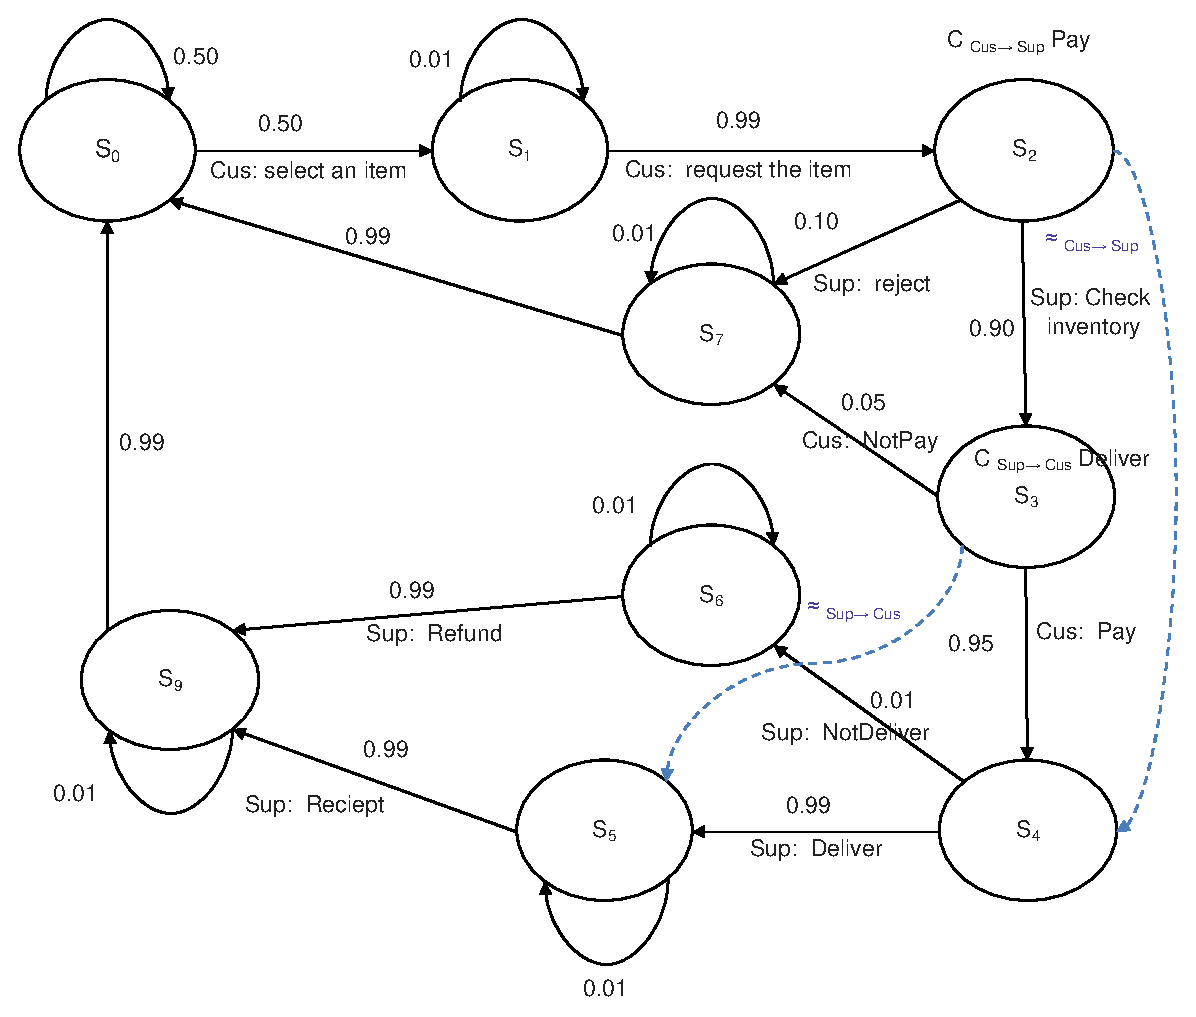
\includegraphics[width=14cm, height=10cm]{chap5/img/online-s-s.eps}
                %height=9cm]{figures/test}
                \end{center}
                \caption{A model for the case of one supplier and one customer} \label{fig:Online-ss}
%                \label{Stack}
                \end{figure}



\subsection{System Properties}\label{sec:properties}

Properties that capture the probabilistic behavior of the online
shopping system have been verified using PRISM in various
proposals, for instance \cite{Ouchani2014}. In this section,
special emphasis is given to properties related to the concepts of
knowledge and social commitments. Concretely, we verify some
system's properties such as \textit{Safety}, \textit{Liveness}, and \textit{Reachability} that involve probabilistic
knowledge, probabilistic commitments, and combinations of both.
For the case of social commitments, our verification covers both
basic and group social commitments. All defined properties are
expressed in PCTL$^{\textrm{kc+}}$.

\begin{itemize}
\item \texttt{Safety Property:} Verifying formulae expressing this property in the system models ensures avoiding the appearance of bad situations in the real systems. One bad situation that need to be verified is when the (Cus) fulfills his commitment to pay for the requested order but the (Sup) does not commit to deliver the requested item. This situation can be expressed in PCTL$^{\textrm{kc+}}$ as follows: \\
$\varphi_2= \mathbb{P}_{\geq1}\Box\neg[\mathbb{P}_{>0} \Diamond
Fu(C_{cus\to sup} (Pay))\wedge \mathbb{P}_{\geq1}\Box\neg
(C_{sup\to cus} (Deliver))]$

\item \texttt{Liveness Property:} In all computation paths it is always the case that if the customer commits to pay for the requested item, then in the future the customer will eventually make the payment. This can be expressed in PCLT$^{\textrm{kc+}}$ as follows:\\
$\varphi_3= \mathbb{P}_{\geq1}[(C_{cus\to sup} (Pay))\supset \mathbb{P}_{\geq1}\Diamond Fu(C_{cus\to sup} (Pay))]$

\item \texttt{Reachability Property:} One possible example with regard to the online shopping system is that if the customer (Cus) commits towards the supplier (Sup) to pay for the requested item, the state at which the customer can fulfill his commitment should be reached from the initial state. That is, there should be a possibility from the initial state for the customer to reach the fulfilment state. This can be formally expressed in PCLT$^{\textrm{kc+}}$ as follows:\\
$\varphi_1= \mathbb{P}_{>0} \Diamond Fu(C_{cus\to sup} (Pay))$.

\end{itemize}

Furthermore, thanks to the probabilistic model clacking technique,
we can also get the satisfiability of given formulae in terms of
quantitative results. That is, checking whether a given formula
holds in the model with a threshold (at least 0.95\% for example)
is achievable. Let us consider the following examples:

\begin{itemize}
    \item Once the customer fulfills his commitment to pay, he will be aware about the payment with at least 0.95\%.\\
      $\varphi_4 = P_{>0.95}~ Fu (C_{cus\to sup} (Pay)) \supset K_{cus} Pay$

    \item Once the customer fulfills his commitment to pay, the supplier will be aware about the payment  with at least 0.98\%.\\
      $\varphi_5 = P_{>0.98}~ Fu (C_{cus\to sup} (Pay)) \supset K_{sup} Pay$
\end{itemize}

%%%%%%%%%%%%%%%%%%%%%%%%%%%%%%%%%%%%%%%%%%%%%%%%%%%%%%%%%%%%%%%%%%%%%%%%%
%%%%%%%%%%%%%%%%%%%%%%%%%%%%%%%%%%%%%%%%%%%%%%%%%%%%%%%%%%%%%%%%%%%%%%%%%

\subsection{Experimental Results}\label{sec:Experimental-results-cha5}

The online shopping system is encoded into the PRISM input
language as follows. Supplier agent (Sup) and Customer agent (Cus)
are mapped into \emph{modules} in the PRISM language. Each agent's
actions are used to determine the behavior of the agent (i.e., his
local states). For example, Supplier's actions (variables) are:
\textit{Accept}: Accept the request, \textit{Reject}: Reject the
request, \textit{Deliver}: Deliver the requested item,
\textit{Receipt}: Send receipt, \textit{Refund}: Refund in case of
not delivery. The global model is obtained by the synchronization
between all modules (agents).

Our implementation was performed on a TOSHIBA laptop equipped with
32-bit Windows XP with 1 GB of RAM and Genuine Intel(R) CPU at 1.6
GHz. Table \ref{Model-Construction-chap5} reports the results of 15
experiments wherein (Exp.\#) denotes the experiment number,
(\#Agent) denotes the number of agents, (\#States) denotes the
number of reachable states, (\#Transitions) denotes the number of
transitions, and (Construction Time) denotes the time needed for
building the simulated model in seconds. \\

First experiment started with only two agents; One supplier (Sup) and one Customer (Cus). In the rest of experiments, we add one more customer (Cus) each time and report the changes occurring in the size of the model and
the time needed for building the model. These results show that (\#States) and (\#Transitions) grow up exponentially as the system is augmented with more agents. However, the (Construction Time) increases polynomially till we reach a point close to the state
explosion, then it grows up dramatically. Figure
\ref{fig:model-time-cha5} shows the increase in the construction
time as more agents join the system. This dramatic change in the
time needed to build the model reflects the fact that the model
size becomes massive.

%\begin{table}[htp][H]
\begin{table}%[H]
\centering \caption{Verification results of the online shopping
system} \label{Model-Construction-chap5}
\resizebox{\textwidth}{!}{ %
\begin{tabular}{|c|c|l|l|c|}
\hline
\texttt{Exp.\#} &   \texttt{\#Agents}    & \texttt{\#States} & \texttt{\#Transitions} & \texttt{Const. Time (s)}\\
\hline\hline
\texttt{Exp.1}   &2             &30            & 74              &0.031\\
\hline
\texttt{Exp.2}   &3             &210           &700              &0.039\\
\hline
\texttt{Exp.3}   &4             &1470          &6102             &0.047\\
\hline
\texttt{Exp.4}   &5           &$1.02*10^{4}$    &$5.10*10^{4}$   &0.063\\
\hline
\texttt{Exp.5}   &6           &$7.20*10^{4}$    &$4.15*10^{5}$   &0.078\\
\hline
\texttt{Exp.6}   &7           &$5.04*10^{5}$    &$3.31*10^{6}$   &0.109\\
\hline
\texttt{Exp.7}   &8           &$3.52*10^{6}$    &$2.60*10^{7}$   &0.189\\
\hline
\texttt{Exp.8}   &9           &$2.47*10^{7}$    &$2.03*10^{8}$   &0.328\\
\hline
\texttt{Exp.9}   &10          &$1.73*10^{8}$    &$1.56*10^{9}$    &0.516\\
\hline
\texttt{Exp.10}  &11          &$1.21*10^{9}$     &$1.19*10^{10}$   &0.765\\
\hline
\texttt{Exp.11}  &12          &$8.47*10^{9}$    &$9.01*10^{10}$   &1.406\\
\hline
\texttt{Exp.12}  &13          &$5.93*10^{10}$   &$6.79*10^{11}$   &2.219\\
\hline
\texttt{Exp.13}  &14          &$4.15*10^{11}$    &$5.09*10^{12}$  &6.094\\
\hline
\texttt{Exp.14}  &15          &$2.91*10^{12}$   &$3.8*10^{13}$    &8.046\\
\hline
\texttt{Exp.15}  &16          &$2.03*10^{13}$  &$2.82*10^{14}$    &13.406\\
\hline
\end{tabular}}
\end{table}



\begin{figure}%[H]
                \begin{center}
                %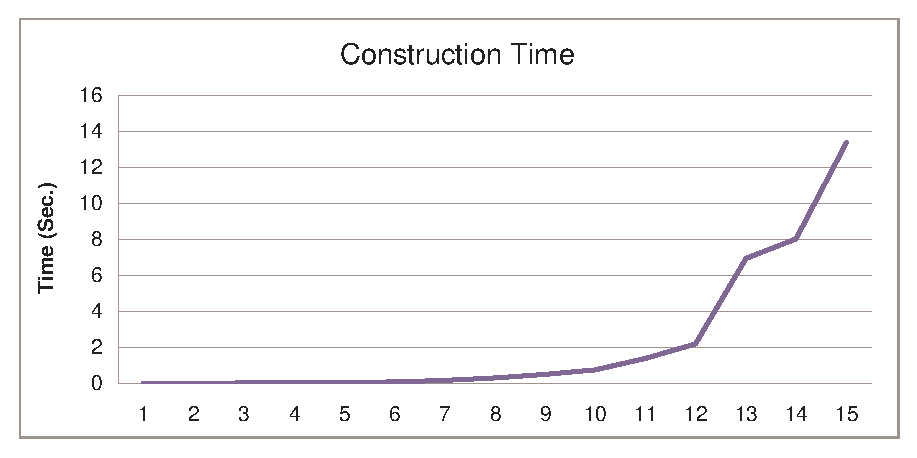
\includegraphics[width=10cm, height=6cm]{chap5/img/construction-time-cha5.eps}
                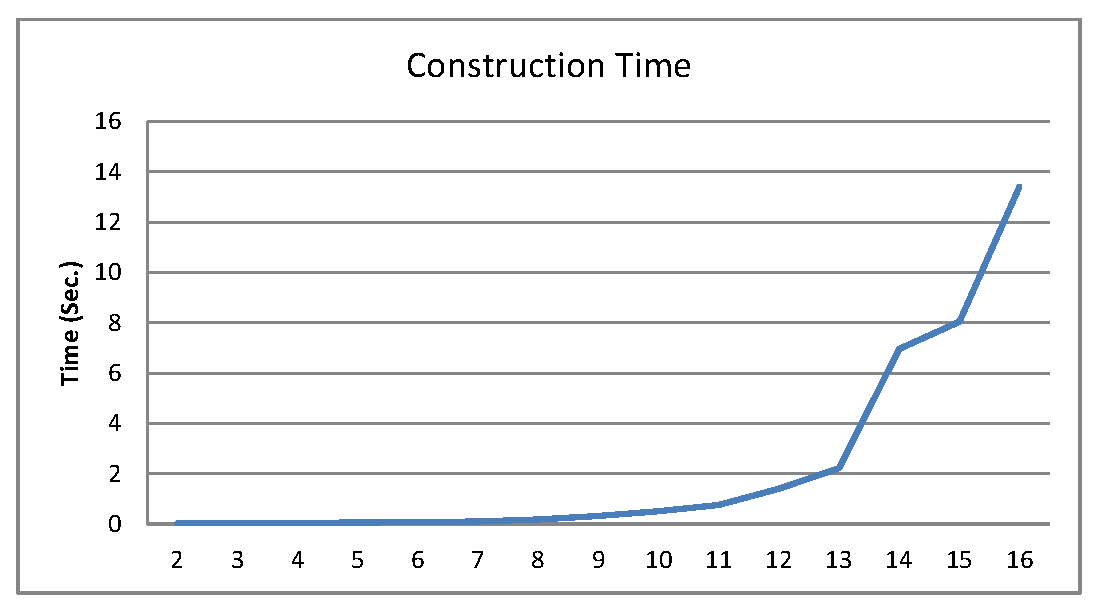
\includegraphics[width=10cm, height=6cm]{chap5/img/time5.eps}
                %height=9cm]{figures/test}
                \end{center}
                \caption{Model construction time for the online shopping system} \label{fig:model-time-cha5}
%                \label{Stack}
                \end{figure}


Table \ref{formulae-prism-results-cha5} reports the model checking
results for the defined formulae ($\varphi_1$ to $\varphi_5$) for
the case of two agents (one customer and one supplier). All
formulae hold in the model as expected, which reflects the success
of our proposed model checking technique in verifying the system
properties expressed using the probabilistic logic
PCTL$^{\textrm{kc+}}$. Moreover, as shown in Table
\ref{formulae-prism-results-cha5}, although the model checking
time varies from one formula to another, it is still short
compared to the time needed for building the model.

For scalability purposes, starting from experiment \#2, we re-write the above-defined formulae in a parameterized form as follows:


$\varphi_1'= \mathbb{P}_{>0} \Diamond \bigwedge\limits_{i=1}^n Fu(C_{cus_i\to sup} (Pay_i))$.

$\varphi_2'= \mathbb{P}_{\geq1}\Box\neg[\mathbb{P}_{>0} \Diamond \bigwedge\limits_{i=1}^n
Fu(C_{cus_i\to sup} (Pay_i))\wedge \mathbb{P}_{\geq1}\Box\neg
(C_{sup\to cus_i} (Deliver_i))]$

$\varphi_3'= \mathbb{P}_{\geq1}[\bigwedge\limits_{i=1}^n (C_{cus_i\to sup} (Pay_i))\supset \mathbb{P}_{\geq1}\Diamond Fu(C_{cus_i\to sup} (Pay_i))]$

$\varphi_4' = P_{>0.95}~ \bigwedge\limits_{i=1}^n Fu (C_{cus_i\to sup} (Pay_i)) \supset K_{cus_i} Pay_i$

$\varphi_5' = P_{>0.98}~ \bigwedge\limits_{i=1}^n Fu (C_{cus_i\to sup} (Pay_i)) \supset K_{sup}
Pay_i$\\
%
where $n$ is the number of agents in the experiment.

\begin{table}%[H]
\centering \caption{Results of model checking some properties for the online shopping system} \label{formulae-prism-results-cha5}
\begin{tabular}{|c|c|c|}
\hline
\texttt{Formulae} &   \texttt{Results}    & \texttt{Time for MC (Sec.)} \\
\hline\hline
$\varphi_1$                &true           &0.06  \\
\hline
$\varphi_2$                &true           &0.13  \\
\hline
$\varphi_3$                &true           &0.11  \\
\hline
$\varphi_4$                &true           &0.06  \\
\hline
$\varphi_5$                &true           &0.07  \\
\hline
\end{tabular}
\end{table}


To be able to verify group social commitments, which is one of the
main motivations of this chapter, we need models of one supplier
agent interacting with two or more customer agents by means of
social commitments. Table \ref{formulae-prism-group-comm-cha5}
reports the results of verifying group social commitments for
experiment \#2 and experiment \#3 using the proposed
reduction technique. In experiment \#2, we have one supplier (Sup) committing to two customers (Cus$_1$) and (Cus$_2$) to deliver the goods. The commitment should be fulfilled in the future to meet the liveness property. Likewise, in experiment \#3, we have one supplier (Sup) committing to three customers (Cus$_1$), (Cus$_2$), and (Cus$_3$) to deliver the requested items.

\noindent $\varphi_6= \mathbb{P}_{\geq1}[(C_{sup \to \{cus_1,cus_2\}} (Deliver))\supset \mathbb{P}_{\geq1}\Diamond Fu(C_{sup \to \{cus_1,cus_2\}} (Deliver))]$

\noindent $\varphi_7= \mathbb{P}_{\geq1}[(C_{sup \to \{cus_1,cus_2,cus_3\}} (Deliver))\supset \mathbb{P}_{\geq1}\Diamond Fu(C_{sup \to \{cus_1,cus_2,cus_3\}} (Deliver))]$

\noindent We were also successful in verifying formulae expressing the interaction between knowledge and group social commitments for experiment \#2 and experiment \#3 as shown below.

\noindent $\varphi_8 = \mathbb{P}_{\geq1}[Fu (C_{sup \to \{cus_1,cus_2\}} (Deliver)) \supset K_{cus_1} (Deliver) \wedge  K_{cus_2} (Deliver)$]

\noindent $\varphi_9 = \mathbb{P}_{\geq1}[Fu (C_{sup \to \{cus_1,cus_2,cus_3\}} (Deliver)) \supset K_{cus_1} (Deliver) \wedge  K_{cus_2} (Deliver) \wedge  K_{cus_3} (Deliver)$]\\

Where, $\varphi_8$ states that the fulfilment of a group commitment (the commitment from $sup$ to $cus_1$ and $cus_2$ to deliver) implies that every creditor in the group will know about the content of the commitment (i.e., $cus_1$ and $cus_2$ will know about the delivery). Similarly, $\varphi_9$ states the same meaning in the case when $sup$ fulfills its commitment to three customers.

\begin{table}[htp]
\centering \caption{Model checking group commitment formulae} \label{formulae-prism-group-comm-cha5}
\begin{tabular}{|c|c|c|c|}
\hline
\texttt{Exp.\#}  &\texttt{\#Agents}  &\texttt{Formulae} &\texttt{Results} \\
\hline\hline
Exp.2            & 1 Sup, 2 Cus      &$\varphi_6$           &true  \\
\hline
Exp.3            & 1 Sup, 3 Cus      &$\varphi_7$           &true  \\
\hline
Exp.2            & 1 Sup, 2 Cus      &$\varphi_8$           &true  \\
\hline
Exp.3            & 1 Sup, 3 Cus      &$\varphi_9$           &true  \\
\hline

\end{tabular}
\end{table}

%%%%%%%%%%%%%%%%%%%%%%%%%%%%%%%%%%%%%%%%%%%%%%%%%%%%

\section{Summary}\label{sec:conclusion}

In this chapter, we introduced a formal approach for specifying and
verifying the interactions between basic (individual) and group social commitments and knowledge in probabilistic MASs. The
proposed approach encompasses three main parts. In the first
part, we presented a new probabilistic logic of knowledge and
commitments (PCLT$^{\textrm{kc+}}$). The expressive power of
PCLT$^{\textrm{kc+}}$ outperforms those of existing logics because
of its ability to express and specify not only the concepts of
knowledge and social commitments independently, but also their
interactions in the presence of uncertainty. Also, being enriched
by operators for the group knowledge and group commitments,
PCLT$^{\textrm{kc+}}$ allows handling more complicated commitment
scenarios with respect to the number of participating agents. We
categorized social commitments into two classes based on the
number of participating agents; basic social commitment (the
common one-to-one scheme) and group social commitment (one-to-many
scheme). We then presented a formal semantics for the group social
commitment. With such a classification of social commitments, we
gain an insight into different ways to utilize commitments among
communicating parties. In contrast, exiting solutions for social commitments restrict themselves to the common one-to-one commitment scheme.

In the second part, we proposed a sound and complete reduction-based model checking technique for the new logic. The proposed technique consists of reducing the problem of model checking PCLT$^{\textrm{kc+}}$ to the problem of model checking PCTL. The soundness and completeness of the reduction technique were proven. Finally, in the third part, we used the
PRISM tool to implement our reduction technique and check
PCLT$^{\textrm{kc+}}$ formulae by checking their corresponding
PCTL formulae without adding new computation cost. In terms of scalability, we showed that our reduction technique is scalable as we were
successfully able to apply it on models of size up to $10^{13}$
states and $10^{14}$ transitions. To conclude, the two main findings of this chapter are:
 \begin{enumerate}
 \item Simply combining a probabilistic logic of knowledge and a probabilistic logic of commitments to capture the interactions between the concept of knowledge and social commitments in probabilistic MASs is not quite working as excepted.
 \item Representing group social commitments and the interactions between group social commitments and knowledge in the presence of uncertainty become attainable by the use of our proposed framework.
 \end{enumerate}

